\documentclass[aspectratio=169]{beamer}
\usepackage{ITMOtheme}
\usepackage{amsmath}
\usepackage{amssymb}
\usepackage{graphicx} % For including images if needed
\usepackage{amsfonts} % For \mathbb symbols
% pt produsu cartezian
\usepackage{mathabx}
\usepackage{mathtools}
\usepackage[backend=biber,
backref=true]{biblatex}
\addbibresource{references.bib}

\usepackage{xcolor}
\usepackage{listings}

%New colors defined below
\definecolor{codegreen}{rgb}{0,0.6,0}
\definecolor{codegray}{rgb}{0.5,0.5,0.5}
\definecolor{codepurple}{rgb}{0.58,0,0.82}
\definecolor{backcolour}{rgb}{0.95,0.95,0.92}

%Code listing style named "mystyle"
\lstdefinestyle{mystyle}{
	backgroundcolor=\color{backcolour}, commentstyle=\color{codegreen},
	keywordstyle=\color{magenta},
	numberstyle=\tiny\color{codegray},
	stringstyle=\color{codepurple},
	basicstyle=\ttfamily\footnotesize,
	breakatwhitespace=false,
	breaklines=true,
	captionpos=b,
	keepspaces=true,
	numbers=left,
	numbersep=5pt,
	showspaces=false,
	showstringspaces=false,
	showtabs=false,
	tabsize=2
}

%"mystyle" code listing set
\lstset{style=mystyle}

\usepackage{minted}
\setminted{python3=true}

\setcounter{biburlnumpenalty}{9000} % Allow breaks after numbers
\setcounter{biburlucpenalty}{9000} % Allow breaks after uppercase letters
\setcounter{biburllcpenalty}{9000} % Allow breaks after lowercase letters

\makeatletter
\newcommand*{\rom}[1]{\expandafter\@slowromancap\romannumeral #1@)}
\makeatother

% sa pot sa fac modulul cu 2 bari gen normu
\DeclarePairedDelimiter\abs{\lvert}{\rvert}%
\DeclarePairedDelimiter\norm{\lVert}{\rVert}%

% Swap the definition of \abs* and \norm*, so that \abs
% and \norm resizes the size of the brackets, and the
% starred version does not.
\makeatletter
\let\oldabs\abs
\def\abs{\@ifstar{\oldabs}{\oldabs*}}
%
\let\oldnorm\norm
\def\norm{\@ifstar{\oldnorm}{\oldnorm*}}
\makeatother

% If ITMOtheme is not used, define some colors for consistency or use standard beamer colors
% \definecolor{ITMOblue}{RGB}{0,70,132}
% \definecolor{ITMOred}{RGB}{200,0,0}

\title[Hopf Bifurcations in CRNs]{Proving existence and ruling out of Hopf bifurcations in Phosphorylation–Dephosphorylation reaction networks}
\author{Stan Ioan-Victor \\[3mm] Lect. dr. Parajdi Lorand}
\date{\today}
\institute{UBB MIE3}

\AtBeginSection[]
{
\begin{frame}
	\frametitle{Presentation Outline}
	\tableofcontents[currentsection]
\end{frame}
}

\begin{document}

\begin{frame}[plain]
\titlepage
\end{frame}

\begin{frame}{Presentation Outline}
\tableofcontents
\end{frame}

% --- Section 1: Why Study Chemical Networks? ---
\section{Thesis summary}

\begin{frame}{\insertsectionhead}
\frametitle{Summary of the Thesis}
\begin{itemize}
	\item Many biological processes are not static; they \alert{oscillate} or cycle over time. Think of:
		\begin{itemize}
			\item \textbf{Circadian Rhythms:} Our internal 24-hour body clocks regulating sleep-wake cycles, hormone release, and metabolism.
			\item \textbf{Heartbeat \& Respiration:} Essential life-sustaining rhythmic activities.
			\item \textbf{Cell Cycle:} The ordered series of events leading to cell division and duplication.
			\item \textbf{Hormonal Cycles:} Regular fluctuations in hormone levels (e.g., menstrual cycle).
		\end{itemize}
	\item These cycles are often driven by networks of interacting molecules - \alert{Chemical Reaction Networks (CRNs)}.
	\item We introduce all the theoretical background needed to understand our analysis.
\end{itemize}
\end{frame}

\begin{frame}{\insertsectionhead}
\frametitle{Phosphorylation: A Key Regulator}
\begin{itemize}
		\small
	\item \alert{Phosphorylation} (adding a phosphate group to a protein) and \alert{dephosphorylation} (removing it) are like molecular on/off switches.
	\item They are fundamental to \alert{cellular communication (signal transduction)}, controlling a vast array of cellular processes:
		\begin{itemize}
			\item Growth, development, and division.
			\item Responses to environmental cues.
			\item Immune responses.
		\end{itemize}
	\item \alert{Dysregulation} in these signaling pathways and their rhythms is implicated in many diseases:
		\begin{itemize}
			\item Cancer (uncontrolled cell growth).
			\item Diabetes (problems with insulin signaling).
			\item Neurological disorders.
			\item Inflammatory diseases.
		\end{itemize}
	\item Studying \alert{Hopf bifurcations} in these (de)phosphorylation CRNs helps us understand how these systems can switch from stable states to oscillatory behavior, providing insights into both normal function and disease mechanisms.
\end{itemize}
\textbf{The thesis was also presented at the Student Scientific Communication Session in Mathematics, on May 24th, 2025.}

\begin{figure}[H]
	\centering
	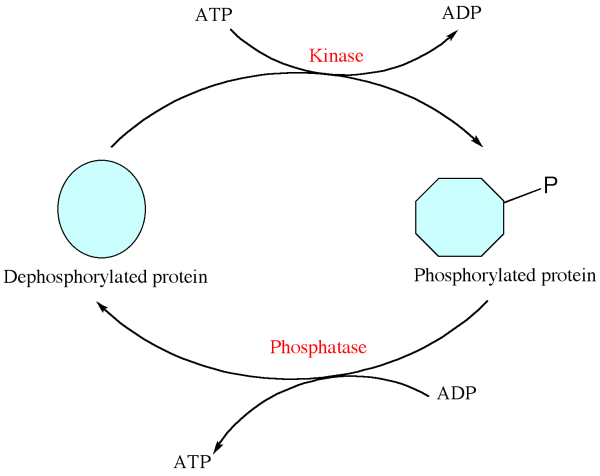
\includegraphics[width=0.5\linewidth]{pics/phosphorylation.png}
	\caption{Phosphorylation from \cite{raimi2014partial}}
\end{figure}
\end{frame}

% --- Section 2: Introduction to Chemical Reaction Networks (CRNs) ---
\section{Introduction to Chemical Reaction Networks (CRNs)}

\begin{frame}{\insertsectionhead}
\frametitle{What is a Chemical Reaction Network (CRN)?}
(thanks to my Proffesor's presentation \cite{Parajdi2024})A CRN consists of:
\begin{itemize}
	\item A set of $\left|S\right| = n$ chemical \alert{species} $S = \{X_1, \dots, X_n\}$.
	\item A set of $r$ \alert{reactions}, each of the form:
		\[
			\alpha_{1j} X_1 + \dots + \alpha_{n j} X_n \xrightarrow{k_j} \beta_{1j} X_1 + \dots + \beta_{n j}, \forall j = \overline{1,r}.	
		\]
	\item $\alpha_{ij}, \beta_{ij} \in \mathbb{N}$ are \alert{stoichiometric coefficients} (stoichiometries) of reactants, respectively products.
	\item $k_j > 0$ are the \alert{reaction rate constants}.
	\item Concentrations are $x = (x_1, \dots, x_n)^T$, where $x_i = [X_i]$.
\end{itemize}
\end{frame}

\begin{frame}{\insertsectionhead}
\frametitle{Mass-Action Kinetics \& ODE Model}
\begin{itemize}
	\item The \alert{rate} of a certain reaction $j$ (mass-action):
		$$ 	v_j : \mathbb{R}^r_{> 0} \bigtimes \mathbb{R}^n_{\geq 0} \rightarrow \mathbb{R}_{\geq 0}   $$
		$$ v_j(k,x) = k_j \prod_{i=1}^{n} x_i^{\alpha_{ij}} $$

	\item The \alert{flux vector} $v : \mathbb{R}^r_{> 0}  \bigtimes \mathbb{R}^n_{\geq 0} \rightarrow \mathbb{R}^r_{\geq 0}$:
		$$ 	(v(x,k))_{i} = v_i(k_i, x)$$
	\item The \alert{left / right stoichiometric matrices} $		\Gamma_L, \Gamma_R \in \mathcal{M}_{n \bigtimes r}(\mathbb{N}), 		(\Gamma_L)_{ij} = \alpha_{ij};
		(\Gamma_R)_{ij} = \beta{ij} $
	\item The \alert{stoichiometric matrix} $\Gamma \in \mathcal{M}_{n \times r}(\mathbb{Z})$: $\Gamma_{ij} = \beta_{ij} - \alpha_{ij}$ (net change).

\end{itemize}
\end{frame}

% --- Section 3: Dynamical Systems Fundamentals ---
\section{Dynamical Systems Fundamentals}

\begin{frame}
\begin{itemize}
	\item Dynamics via Ordinary Differential Equations (ODEs):
		$$ \frac{dx}{dt} = \Gamma \cdot v(k,x) $$
		This system models how concentrations change over time.

		Take this \textbf{open network} as an example:
\end{itemize}
\begin{align*}
	A + C \xrightarrow{k_{1}} 2A \\
	B + C \xrightarrow{k_{2}} 2B  \\
	A \xrightarrow{k_{3}} 0 \\
	B \xrightarrow{k_{4}} 0 \\
	0 \xrightarrow{k_{5}} C
\end{align*}
\end{frame}

\begin{frame}
The stoichiometric matrices:
\begin{align*}
	\Gamma_L =
	\begin{pmatrix}
		1 & 0 & 1 & 0 & 0 \\
		0 & 1 & 0 & 1 & 0 \\
		1 & 1 & 0 & 0 & 0
	\end{pmatrix}
	, \quad
	\Gamma_R =
	\begin{pmatrix}
		2 & 0 & 0 & 0 & 0 \\
		0 & 2 & 0 & 0 & 0 \\
		0 & 0 & 0 & 0 & 1
	\end{pmatrix}
\end{align*}
\begin{equation*}
	\Gamma =
	\begin{pmatrix*}
		1 & 0 & -1 & 0 & 0 \\
		0 & 1 & 0 & -1 & 0 \\
		-1 & -1 & 0 & 0 & 1
	\end{pmatrix*}
\end{equation*}
Whereas, the reaction rate (\textbf{flux vector}):
\[
	v(k,x) =
	\begin{pmatrix*}
		v_{1}(k,x)	 \\
		v_{2}(k,x)	 \\
		v_{3}(k,x)	 \\
		v_{4}(k,x)	 \\
		v_{5}(k,x)
	\end{pmatrix*} =
	\begin{pmatrix}
		k_1 x_1 x_3 \\
		k_2 x_2 x_3 \\
		k_3 x_1 \\
		k_4 x_2 \\
		k_5
	\end{pmatrix}
\]
\end{frame}

\begin{frame}
And so its dynamical system in matrix form is:
\begin{align*}
	\frac{dx}{dt} &= \Gamma v(k,x) \\
	\frac{d}{dt}
	\begin{pmatrix*}
		x_1	\\
		x_2	\\
		x_3	
	\end{pmatrix*} &=
	\begin{pmatrix*}
		1 & 0 & -1 & 0 & 0 \\
		0 & 1 & 0 & -1 & 0 \\
		-1 & -1 & 0 & 0 & 1
	\end{pmatrix*}
	\begin{pmatrix}
		k_1 x_1 x_3 \\
		k_2 x_2 x_3 \\
		k_3 x_1 \\
		k_4 x_2 \\
		k_5
	\end{pmatrix}
\end{align*}
Resulting in the ODE system:
\[
	\begin{cases*}
		\dot{x}_1 = k_1 x_1 x_3 - k_3x_1  \\
		\dot{x}_2 = k_2 x_2 x_3 - k_4 x_2  \\
		\dot{x}_3 = -k_1 x_1 x_3 - k_2 x_2 x_3 + k_5 \\
	\end{cases*}
\]
\end{frame}

\begin{frame}{\insertsectionhead}
\frametitle{Dynamical Systems: State, Flow, Orbits}
A dynamical system $(T, S, \Phi)$ involves:
\begin{itemize}
	\item $T$: Time (e.g., $\mathbb{R}_{\ge 0}$).
	\item $S$: State space (e.g., possible concentrations, $\mathbb{R}^n_{>0}$).
	\item $\Phi$: Evolution function $\Phi(t, s_0)$ gives the state at time $t$ starting from $s_0$.
		\begin{itemize}
			\item $\Phi(0, s) = s$.
			\item $\Phi(t_2, \Phi(t_1, s)) = \Phi(t_1+t_2, s)$.
		\end{itemize}
	\item The \alert{flow} through $s_0$ is $\Phi_{s_0}(t) = \Phi(t,s_0)$.
	\item The \alert{orbit} (or trajectory) $\gamma_{s_0}$ is the image of the flow: $\{\Phi(t,s_0) | t \in T\}$.
	\item An \alert{invariant set} $\mathcal{M} \subseteq S$ is s.t. $\forall s_0 \in \mathcal{M} \implies \Phi(t,s_0) \in \mathcal{M}, \forall t \ge 0$.
\end{itemize}
\end{frame}

\begin{frame}
\centering
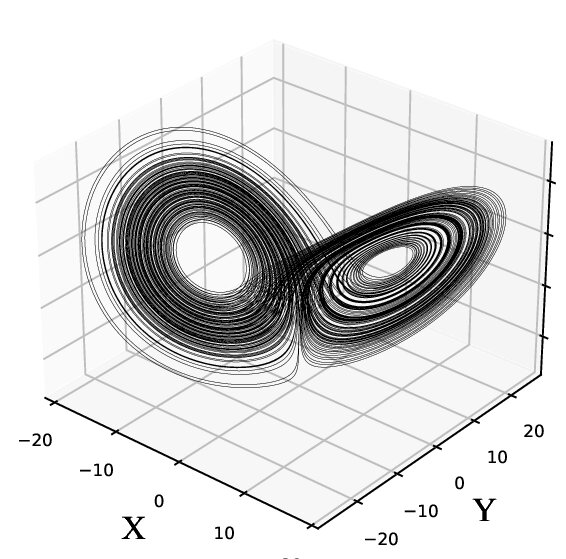
\includegraphics[width=0.6\linewidth]{pics/lorenz.jpg}\\
\end{frame}

\begin{frame}{\insertsectionhead}
\frametitle{Equilibrium Points and Their Stability}
For $\dot{x} = f(x)$:
\begin{itemize}
	\item An \alert{equilibrium point} (steady state) $x^* \in S$ satisfies $f(x^*) = 0$.
		For a CRN: $\Gamma v(k, x^*) = 0$.
	\item \alert{Lyapunov Stability}: $\forall \epsilon > 0, \exists \delta > 0 : 	\text{\rom{1} } \forall x(0) \in S \text{ for which } \norm{x(0) - x^*} < \delta \implies \exists x(t), \forall t >= 0. \quad \text{\rom{2}: } \norm{ x(t) - x^* } < \epsilon \quad \forall t >= 0. $

	\item \alert{Asymptotic Stability}: Additionally: $	\text{\rom{3}: } \lim_{t \rightarrow \infty} \norm{x(t) - x^*}  = 0 \text{ for those whose } \norm{ x(0) - x^*} < \delta$ .These are often called \alert{attractors}.
	\item \alert{Unstable}: If not stable. Solutions may diverge.
\end{itemize}
\end{frame}

\begin{frame}{\insertsectionhead}
\frametitle{Linearization and Eigenvalues}
To analyze stability near an equilibrium $x^*$:
\begin{itemize}
	\item \alert{Linearize} $\dot{x}=f(x)$ around $x^*$: Let $z = x - x^*$. Then $\dot{z} \approx J z$.
	\item The \alert{Jacobian matrix} $J$ at $x^*$: $J_{ij} = \frac{\partial f_i}{\partial x_j} \bigg|_{x^*}$.
	\item \alert{Eigenvalues $\lambda_k$} of $J$ dictate local behavior:
		\begin{itemize}
			\item All Re($\lambda_k$) $< 0 \implies x^*$ is asymptotically stable.
			\item Some Re($\lambda_k$) $> 0 \implies x^*$ is unstable.
			\item Some Re($\lambda_k$) $= 0$ (others $<0$) $\implies x^*$ is non-hyperbolic. \alert{Crucial for bifurcations!} (pretty hard to study given only the linearization).
		\end{itemize}
\end{itemize}
\end{frame}

%  --- Section 4: (De)phosphorylation Cycles: Cellular Switches \& Clocks ---
\section{(De)phosphorylation Cycles: Cellular Switches \& Clocks}

\begin{frame}{\insertsectionhead}
\frametitle{(De)phosphorylation Cycles: Cellular Switches \& Clocks}
\begin{itemize}
	\item (De)phosphorylation cycles are key in \alert{signal transduction}.
	\item Involve: Substrate $S$ (forms $S_0, \dots, S_n$), Kinase $K$, Phosphatase $F$.
	\item Example (single site) $\mathcal{N}_1$:
		\begin{align*}
			S_0 + K &\rightleftharpoons KS_0 \xrightarrow{k_3} S_1 + K \\
			S_1 + F &\rightleftharpoons FS_1 \xrightarrow{k_6} S_0 + F
		\end{align*}
	\item \alert{Key Question}: Can these networks act as \alert{switches} (multiple steady states, bistability) or as \alert{clocks} (sustained oscillations via Hopf)? This determines their functional role.
\end{itemize}
\end{frame}

\begin{frame}{\insertsectionhead}
\frametitle{Types of (De)phosphorylation Mechanisms}
The specific mechanism influences dynamic behavior:
\begin{itemize}
	\item \alert{Distributive}: Enzyme dissociates after each single modification event.
		\begin{itemize}
			\item $S_0 + K \to \dots \to S_1 + K$, then $S_1 + K \to \dots \to S_2 + K$.
		\end{itemize}
	\item \alert{Processive}: Enzyme performs multiple modifications before dissociating.
		\begin{itemize}
			\item $S_0 + K \to S_0K \to S_1K \to \dots \to S_n + K$.
		\end{itemize}
	\item For multi-site phosphorylation (e.g., two sites $S_{ij}$):
		\begin{itemize}
			\item \alert{Sequential}: Last site phosphorylated is first dephosphorylated (e.g., $S_{00} \to S_{10} \to S_{11} \to S_{01} \to S_{00}$).
			\item \alert{Cyclic (ordered)}: First site phosphorylated is first dephosphorylated (e.g., $S_{00} \to S_{10} \to S_{11} \to S_{10 \text{ (F removes from site 1)}} \to S_{00 \text{ (F removes from site 0)}}$ - this is a common depiction but the example from `main.pdf` for N2 is $S_{00} \leftrightarrow S_{10} \leftrightarrow S_{11} \leftrightarrow S_{01} \leftrightarrow S_{00}$).
		\end{itemize}
\end{itemize}
\centering
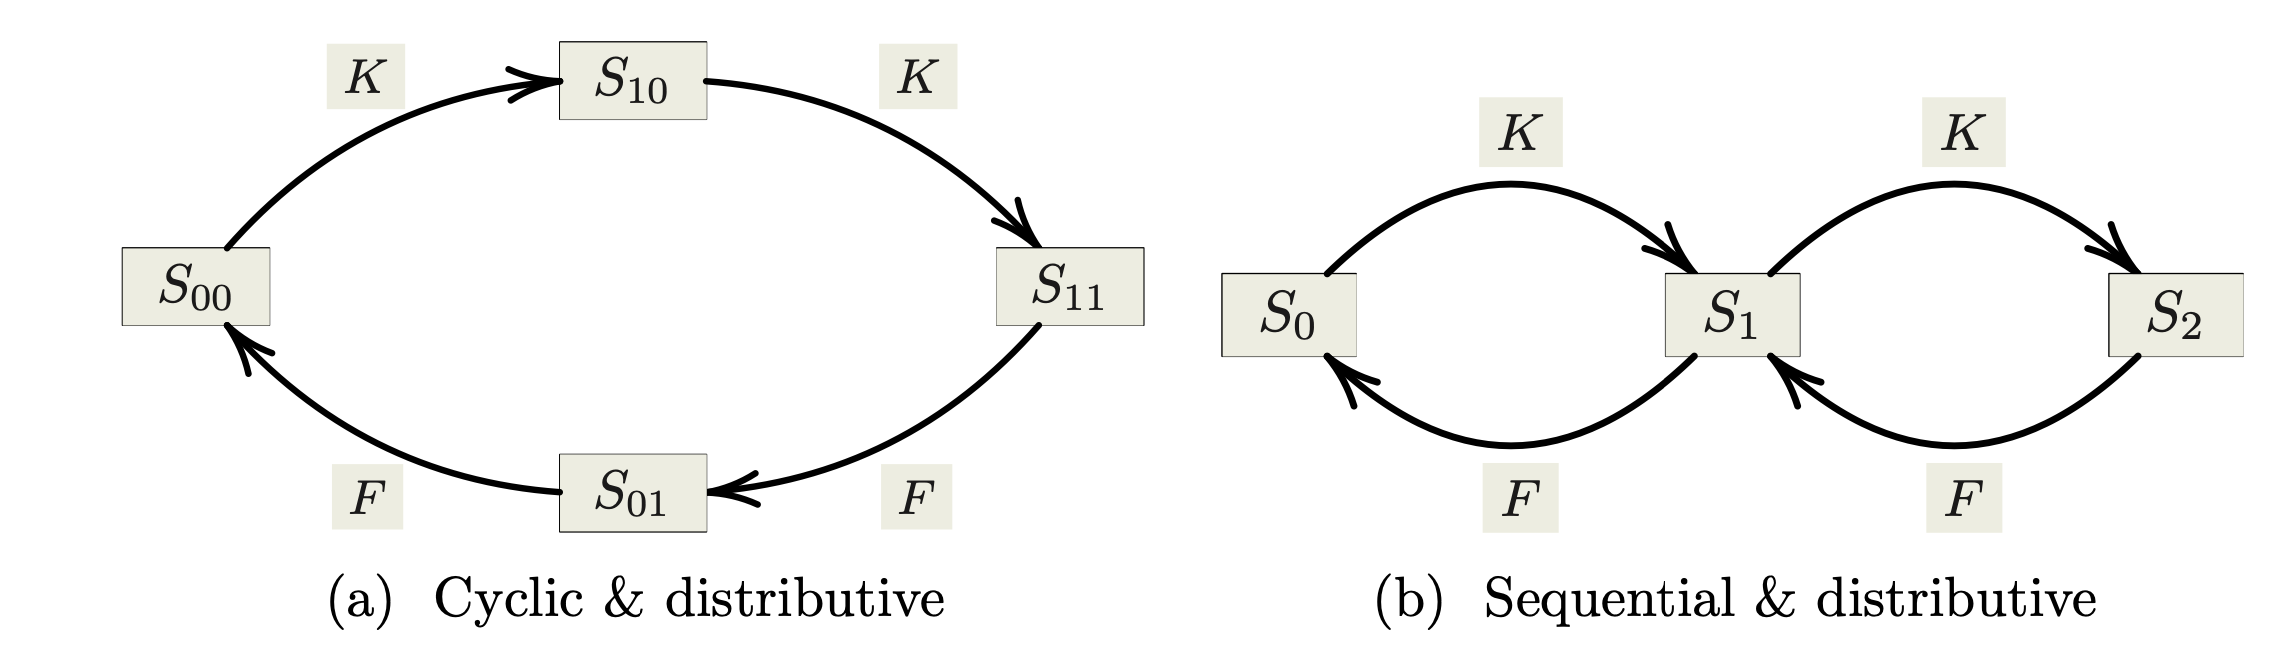
\includegraphics[width=0.6\linewidth]{pics/cyclic-vs-sequential.png} \\
\tiny (Illustrative: Placeholder for Fig (a) and (b) from `main.pdf` section 4.3.1)
\end{frame}

% --- Section 4: Bifurcation Theory ---
\section{Bifurcation Theory}

\begin{frame}{\insertsectionhead}
\frametitle{What is a Bifurcation?}
\begin{itemize}
	\item Consider $\dot{x} = f(x, \mu)$, where $\mu$ is a \alert{bifurcation parameter} (e.g., a rate constant, total amount of an enzyme).
	\item A \alert{bifurcation} occurs at $\mu_0$ if the system's qualitative behavior changes as $\mu$ passes $\mu_0$.
	\item Examples of changes:
		\begin{itemize}
			\item Number or stability of equilibria.
			\item Appearance/disappearance of \alert{periodic orbits (limit cycles)}.
		\end{itemize}
	\item \alert{Local bifurcations} involve changes near an equilibrium and are detected via Jacobian eigenvalues.
	\item Whereas \alert{global bifurcations} involve changes in the system's topology or structure, often requiring more complicated analysis.
\end{itemize}
\end{frame}

\begin{frame}
\centering
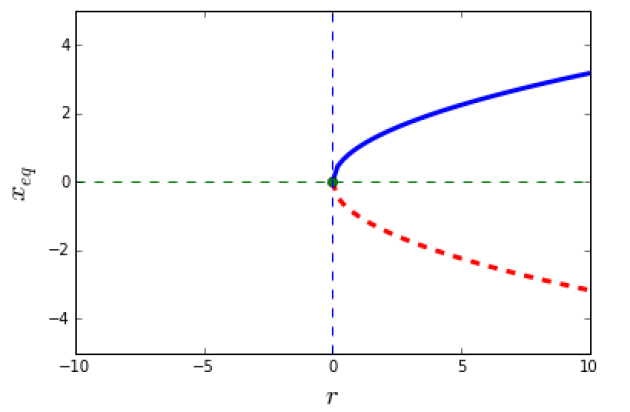
\includegraphics[width=0.8\linewidth]{pics/saddle-node-bif.png}\\
\tiny (Illustrative: Saddle-node bifurcation)
\end{frame}

\begin{frame}
\centering
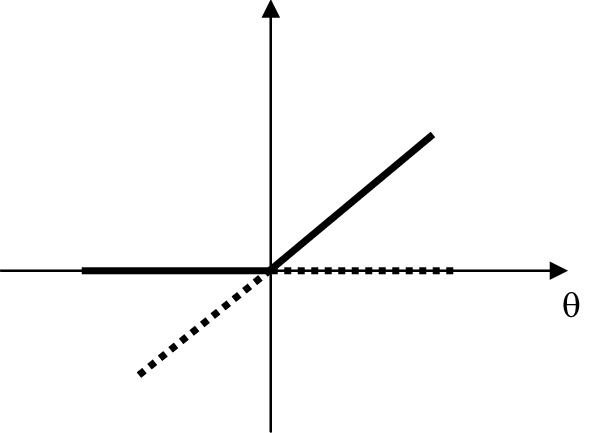
\includegraphics[width=0.8\linewidth]{pics/transcritical-bif.png}\\
\tiny (Illustrative: Transcritical bifurcation)
\end{frame}

\begin{frame}
\centering
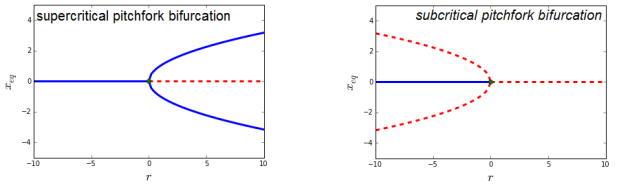
\includegraphics[width=1.01\linewidth]{pics/pitchfork-bif.png}\\
\tiny (Illustrative: Pitchfork bifurcation)
\end{frame}

\begin{frame}{\insertsectionhead}
\frametitle{Hopf Bifurcation: The Birth of Oscillations}
A simple Hopf bifurcation occurs at $(x^*, \mu_0)$ if:
\begin{enumerate}
	\item $J(x^*, \mu_0)$ has a \alert{single pair of complex conjugate eigenvalues} $\lambda_{1,2}(\mu) = \alpha(\mu) \pm i\omega(\mu)$ with:
		\begin{itemize}
			\item $\alpha(\mu_0) = 0$ (purely imaginary at $\mu_0$).
			\item $\omega(\mu_0) \neq 0 \implies \lambda \neq 0$.
		\end{itemize}
	\item All other $n-2$ eigenvalues have Re($\lambda_j$) $< 0$.
	\item \alert{Transversality}: $\frac{d\alpha}{d\mu}\bigg|_{\mu_0} \neq 0$ (eigenvalues).
\end{enumerate}
\alert{Result}: A stable equilibrium can lose stability, giving rise to a stable \alert{limit cycle} (sustained oscillation), or an unstable one can become stable.
\end{frame}

\begin{frame}{\insertsectionhead}
\frametitle{Visualizing a Supercritical Hopf Bifurcation}
As parameter $\mu$ increases through $\mu_0$:
\begin{columns}[T]
	\column{0.5\textwidth}
	\textbf{Eigenvalue Movement:}
	\begin{itemize}
		\item $\mu < \mu_0$: Re($\lambda_{1,2}$) < 0 (stable focus)
		\item $\mu = \mu_0$: Re($\lambda_{1,2}$) = 0 (center-like)
		\item $\mu > \mu_0$: Re($\lambda_{1,2}$) > 0 (unstable focus)
	\end{itemize}
	\centering
	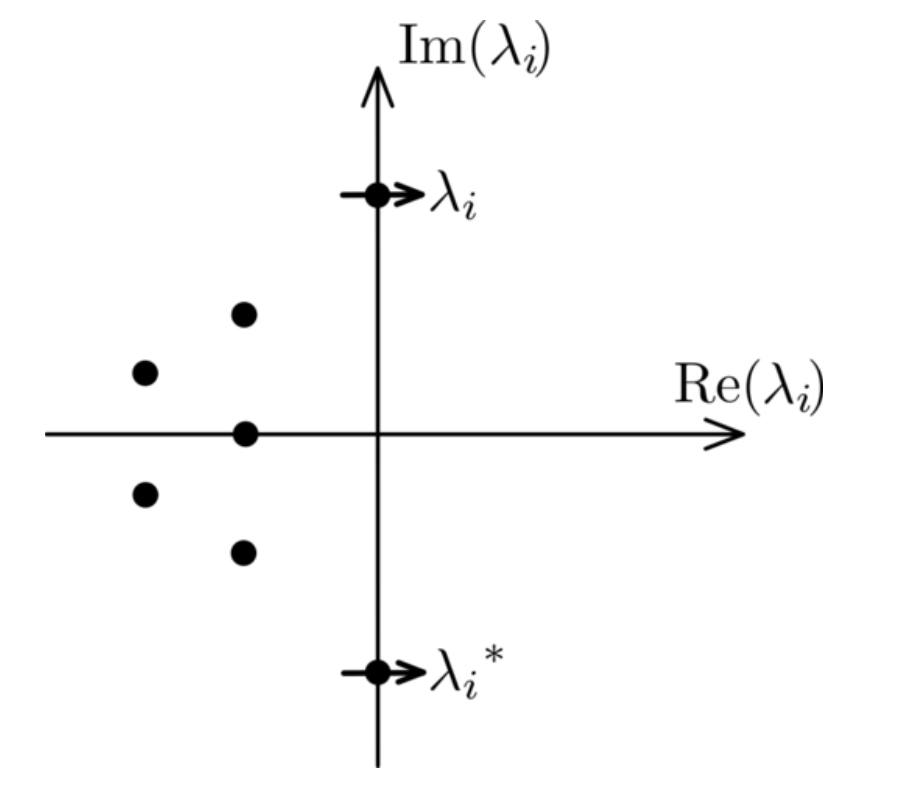
\includegraphics[width=0.8\linewidth]{pics/hopf-bif-eigenvalue-graph.png}\\
	\tiny (Illustrative: Eigenvalues crossing imaginary axis)

	\column{0.5\textwidth}
	\textbf{Phase Portrait Change:}
	\begin{itemize}
		\item $\mu < \mu_0$: Stable equilibrium.
		\item $\mu > \mu_0$: Equilibrium unstable, stable limit cycle appears.
	\end{itemize}
	\centering
	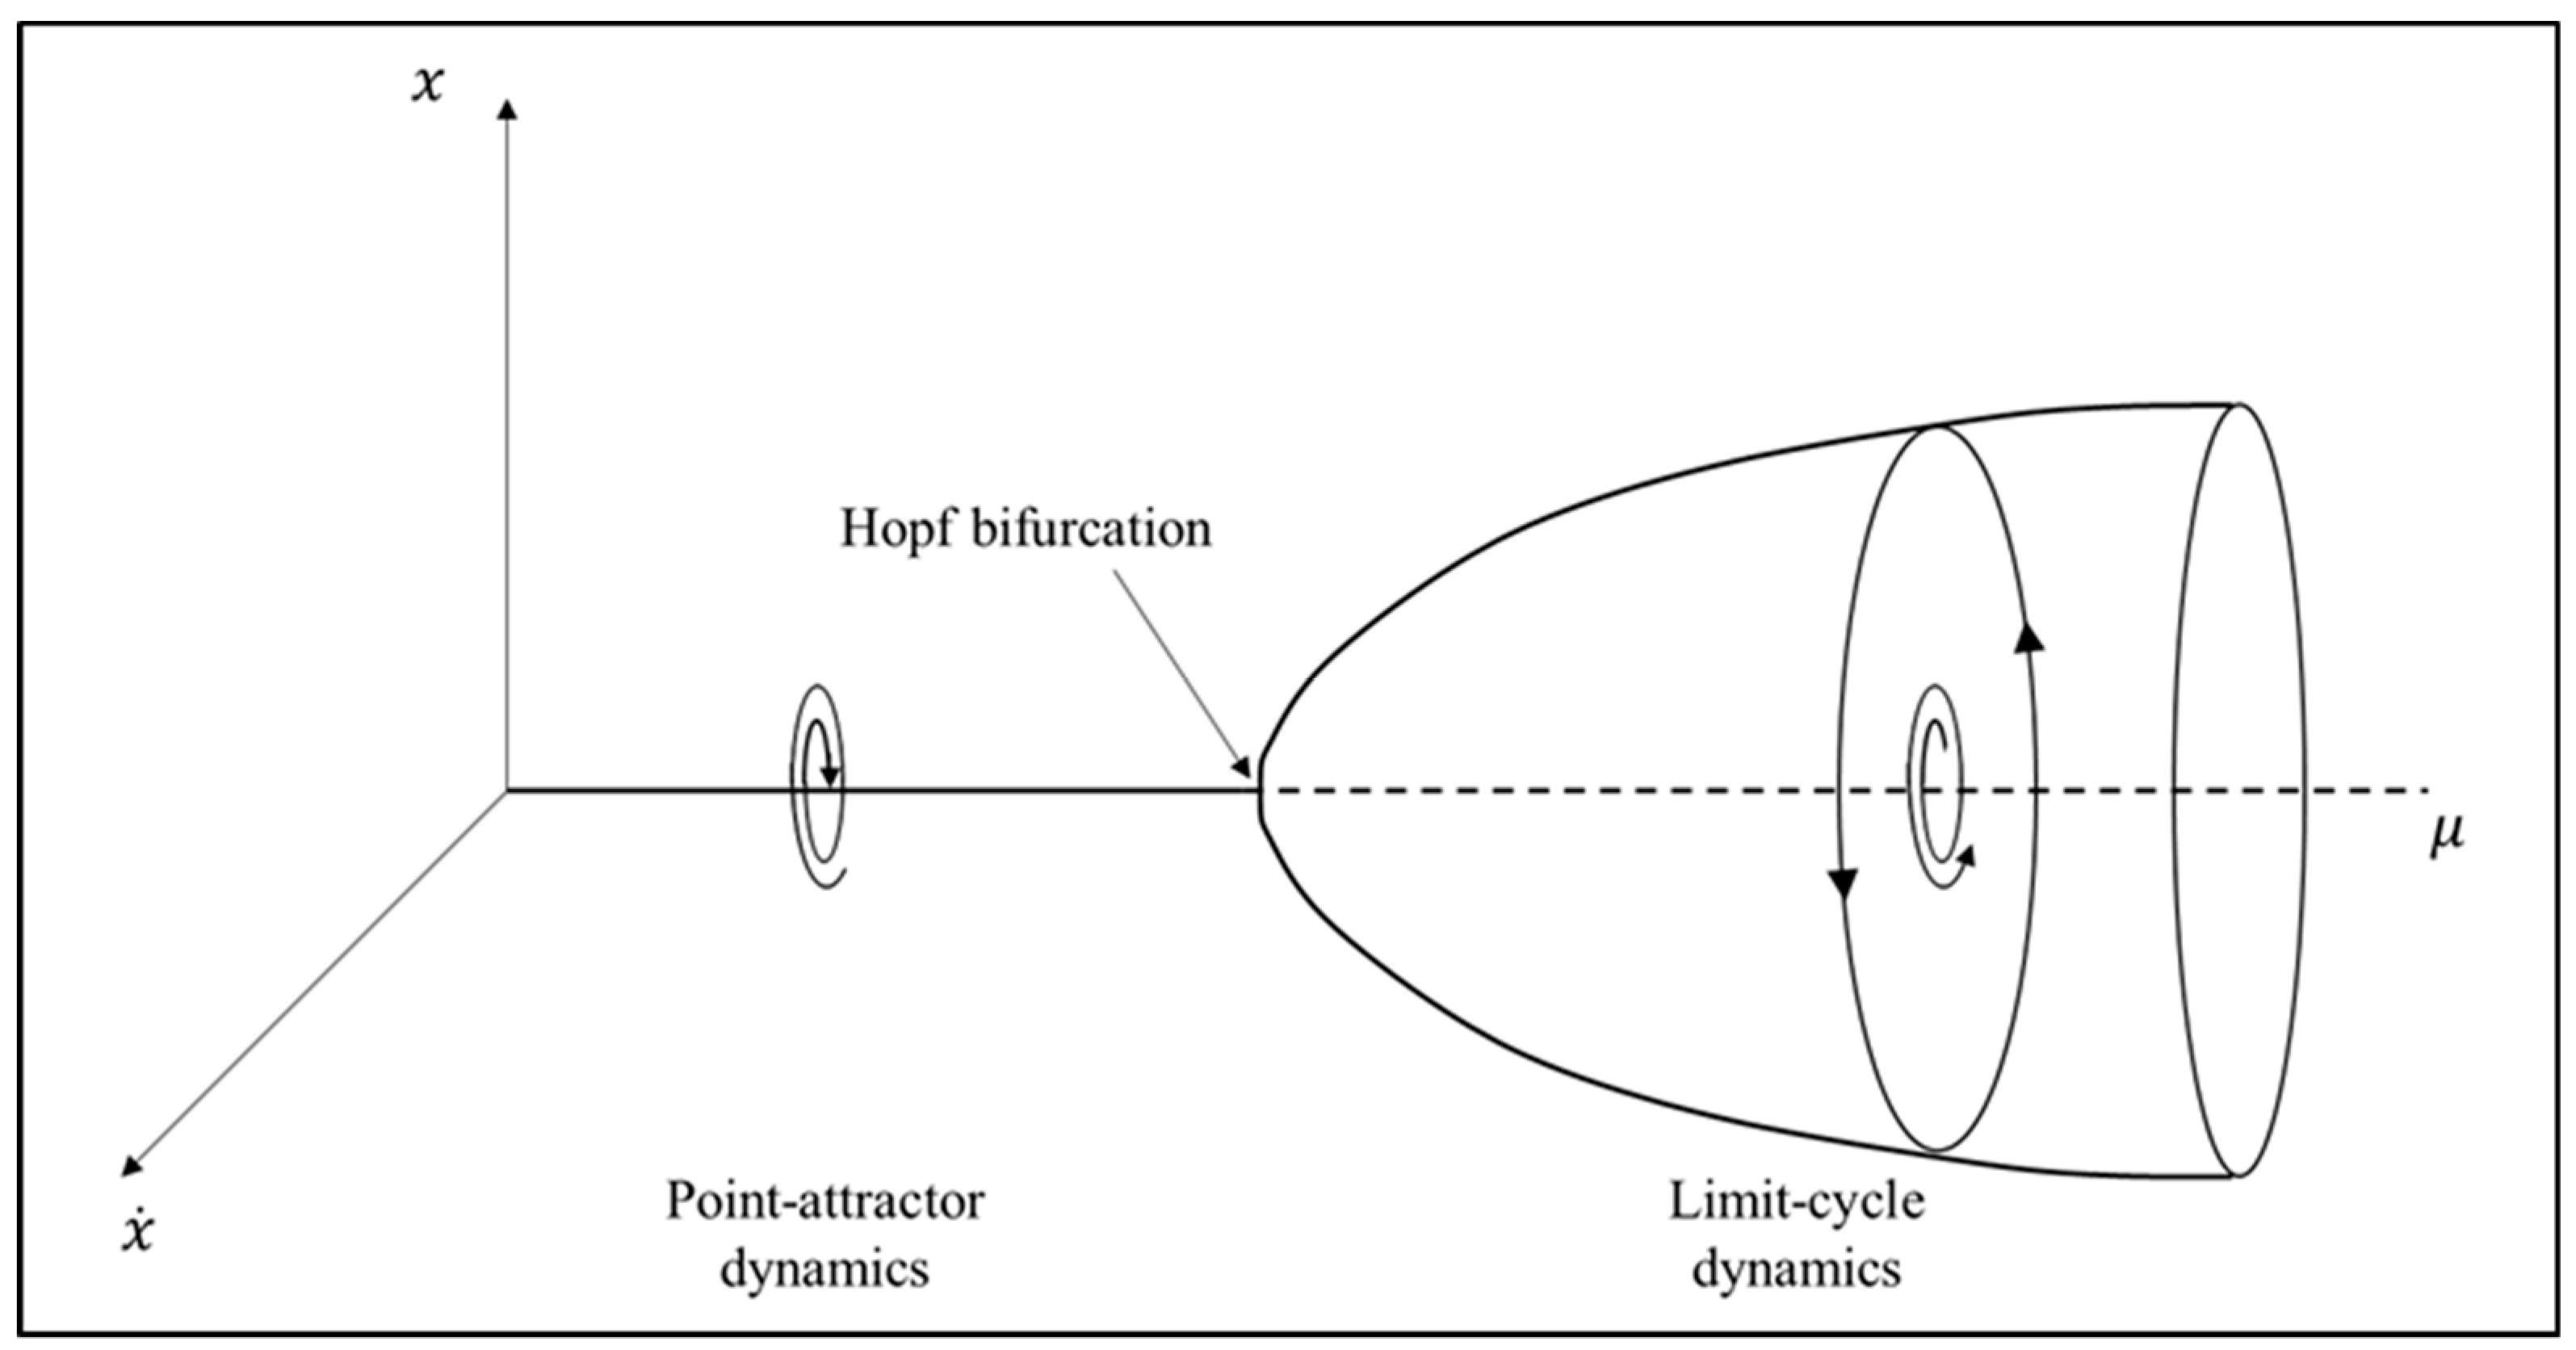
\includegraphics[width=0.8\linewidth]{pics/hopf-bif-pic.png}\\
	\tiny (Illustrative: Birth of a limit cycle \cite{brainsci10080536})
\end{columns}
\vspace{0.5cm}
\small Supercritical: stable limit cycle born. Subcritical: unstable limit cycle merges/destroys stable equilibrium.
\end{frame}

\begin{frame}
So having these in mind, Hopf is kind of like an $\mathbb{R}^n$ version of a Pitchfork bifurcation when you think about it.
You can even see the resemblance in the way they look
\centering
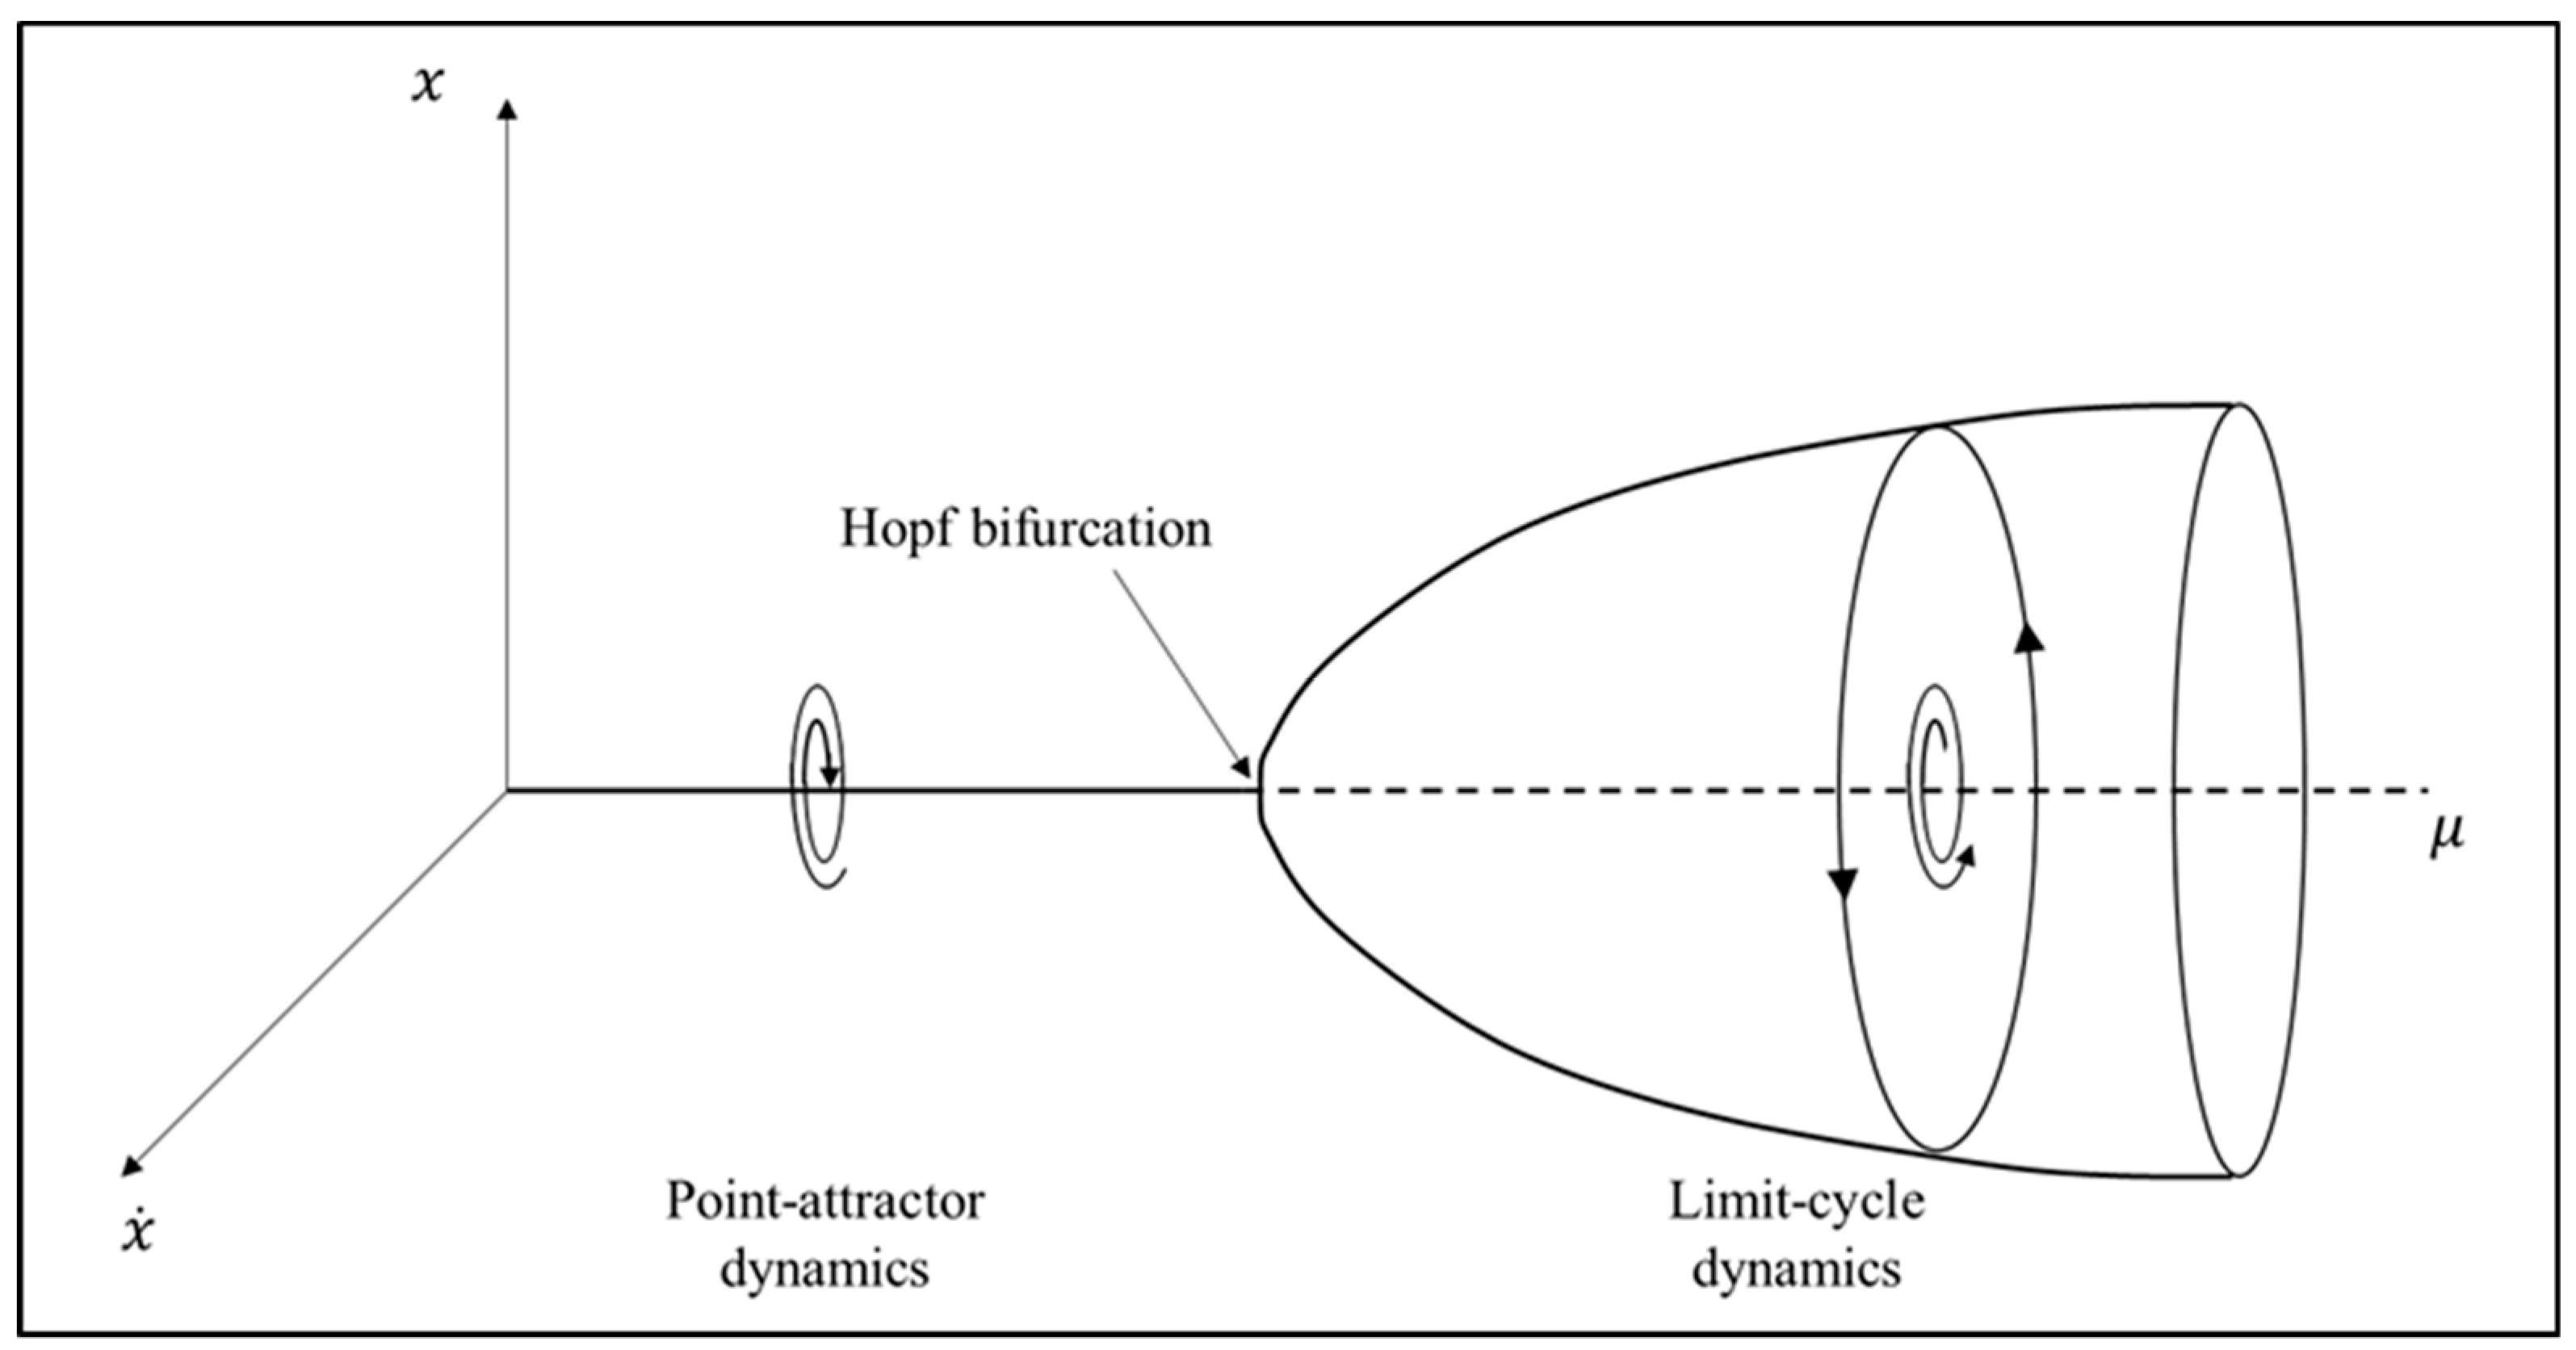
\includegraphics[width=0.8\linewidth]{pics/hopf-bif-pic.png}\\
\tiny (Illustrative: Hopf vs Pitchfork bifurcations)
\end{frame}

\begin{frame}
\centering
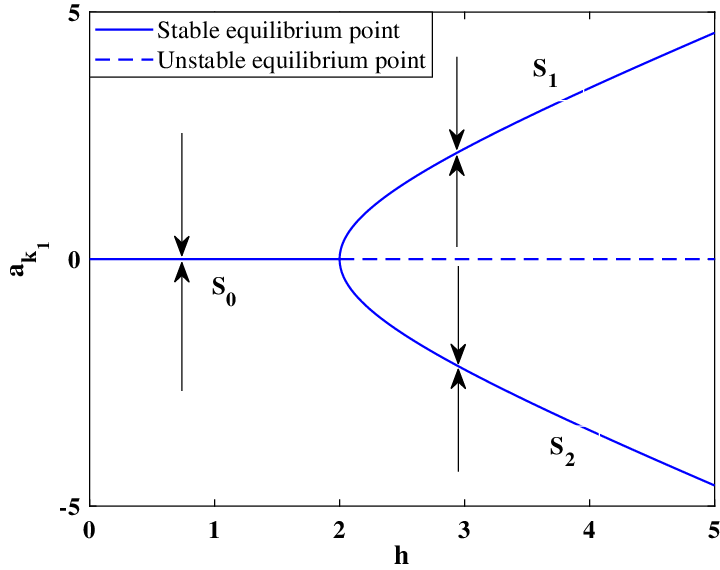
\includegraphics[width=0.7\linewidth]{pics/pitchfork-photo.png}
\end{frame}

% --- Section 5: Detecting Hopf Bifurcations ---
\section{Detecting Hopf Bifurcations}

\begin{frame}{\insertsectionhead}
\frametitle{Characteristic Polynomial \& Routh-Hurwitz}
\begin{itemize}
	\item Characteristic polynomial of $J(\mu)$:
		$$ P(\lambda, \mu) = \det(J(\mu) - \lambda I_n) = a_0\lambda^n + a_1\lambda^{n-1} + \dots + a_n = 0 $$
		(Assume $a_0 > 0$, coefficients $a_i$ depend on $\mu$).
	\item \alert{Routh-Hurwitz criterion}: Conditions on $a_i(\mu)$ for all Re($\lambda_k$) $< 0$.
	\item Involves \alert{Hurwitz matrices} $H_k(\mu)$. For $n$, $H_n(\mu)$:
		$$  H_n(\mu) =
		\begin{pmatrix}
			a_1 & a_3 & a_5 & \dots \\
			a_0 & a_2 & a_4 & \dots \\
			0 & a_1 & a_3 & \dots \\
			\vdots & \vdots & \ddots & \vdots \\
			0 & \dots & \dots & a_n
		\end{pmatrix}
		= (a_{2j - i})_{ij}$$
		($a_k = 0$ if $k<0$ or $k>n$).
	\item Stability $\iff$ all leading principal minors $\Delta_k = \det H_k(\mu)$ are positive: $\det H_i(\mu) > 0, \forall i = \overline{1,n}$.
\end{itemize}
\end{frame}

\begin{frame}{\insertsectionhead}
\frametitle{Criterion for Hopf Bifurcation (Yang)}
For a system of effective degree $s \ge 2$ (after factoring out zero eigenvalues), a simple Hopf bifurcation occurs at $\mu_0$ if:
\begin{enumerate}
	\item $\det H_{s-1}(\mu_0) = 0$.
	\item $\det H_1(\mu_0) > 0, \dots, \det H_{s-2}(\mu_0) > 0$.
	\item $a_s(\mu_0) > 0$ (constant term of the effective characteristic polynomial).
	\item Transversality: $\frac{d}{d\mu}(\det H_{s-1}(\mu))\bigg|_{\mu_0} \neq 0$.
\end{enumerate}
These ensure one pair of purely imaginary eigenvalues crosses the axis, others stable.
\end{frame}

\begin{frame}{\insertsectionhead}\label{thm:rule-out-bifurcations}
\frametitle{(Theorem) Ruling Out Hopf Bifurcations}
No simple Hopf bifurcation along $x^*(\mu)$ if, for all relevant $\mu$:
\begin{itemize}
	\item $\det H_1(\mu) > 0, \dots, \det H_{s-2}(\mu) > 0$ (preliminary stability for other roots),
	\item AND either:
		\begin{itemize}
			\item Whenever $\det H_{s-1}(\mu) = 0 \implies a_s(\mu) \le 0$. (opposes condition 3)
			\item OR, $\det H_{s-1}(\mu) \neq 0$ for all $\mu$. (opposes condition 1)
		\end{itemize}
\end{itemize}
\end{frame}

% --- Section 6: Application to (De)phosphorylation CRNs ---
\section{Solving $\mathcal{N}_1 CRN$}

\begin{frame}{\insertsectionhead}
\frametitle{Convex Parameters for CRN Analysis}
\begin{itemize}
	\item Jacobian $J(k, x^*)$ analysis can be algebraically complex.
	\item \alert{Convex parameterization} $(h, \lambda)$ can simplify $J$:
		\begin{itemize}
			\item $h_i = \frac{1}{x_i^*}$ (inverse steady-state concentrations).
			\item $v^* = E\lambda$ : flux vector, $E$ matrix of extreme rays of flux cone $\text{ker}(\Gamma) \bigcap \mathbb{R}^r_{\ge 0}$, $\lambda$ convex parameters.
			\item $J(h, \lambda) = \Gamma \text{diag}(E\lambda) \Gamma_L^T \text{diag}(h)$ (trick for differentiating).
		\end{itemize}
	\item Coefficients of $J(h,\lambda)$ become \alert{monomials} in $h, \lambda$, simplifying analysis of Hurwitz determinants.
\end{itemize}
\end{frame}

\begin{frame}
% picture insert
\centering
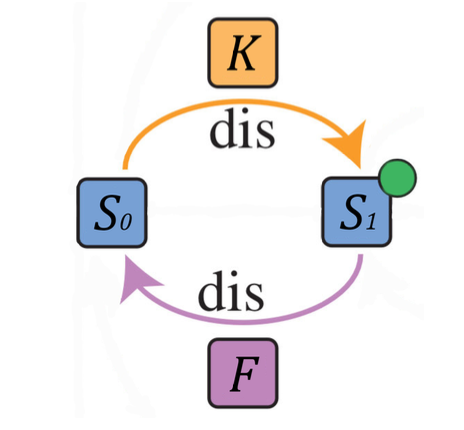
\includegraphics[width=0.5\linewidth]{pics/ex1-no-bifurcations.png} \\ 	

\begin{align*}
	S_0 + K &\rightleftharpoons KS_0 \xrightarrow{k_3} S_1 + K  \tag{$\mathcal{N}_1$} \\
	S_1 + F &\rightleftharpoons FS_1 \xrightarrow{k_6} S_0 + F
\end{align*}
\end{frame}

\begin{frame}{\insertsectionhead}
\frametitle{Example 1: Network $\mathcal{N}_1$ (Basic Cycle)} Using this as example I'll also showcase \href{https://github.com/viktorashi/Open-CoNtRol}{the app} that I've been working on for my thesis.
For $K + S_0 \rightleftharpoons KS_0 \rightarrow K + S_1$, $F + S_1 \rightleftharpoons FS_1 \rightarrow F + S_0$ ($\mathcal{N}_1$):
\begin{align*}
	\Gamma &=
	\begin{pmatrix}
		K & -1 &  1 &  1 &  0 &  0 &  0 \\
		S0& -1 &  1 &  0 &  0 &  0 &  1 \\
		KS0 &  1& -1& -1 &  0 &  0 &  0 \\
		S1 &  0 &  0 &  1& -1 &  1 &  0 \\
		F &  0 &  0 &  0& -1 &  1 &  1 \\
		FS1 &  0 &  0 &  0 &  1& -1& -1  \\		
	\end{pmatrix}, \quad \text{rank}(\Gamma) = 3 \\[3ex]
	\Gamma_L &=
	\begin{bmatrix}
		1&0&0&0&0&0\\
		1&0&0&0&0&0\\
		0&1&1&0&0&0\\
		0&0&0&1&0&0\\
		0&0&0&1&0&0\\
		0&0&0&0&1&1
	\end{bmatrix} \\[3ex]
\end{align*}
\end{frame}

\begin{frame}
\begin{align*}
	\begin{cases*}
		\begin{array}{ll}
			\dot{x}_1(t) = -k_4 x_1(t) x_6(t)+k_5 x_2(t)+k_6 x_2(t) \\
			\dot{x}_2(t) = k_4 x_1(t) x_6(t)-k_5 x_2(t)-k_6 x_2(t) \\
			\dot{x}_3(t) = -k_1 x_3(t) x_5(t)+k_2 x_4(t)+k_3 x_4(t) \\
			\dot{x}_4(t) = k_1 x_3(t) x_5(t)-k_2 x_4(t)-k_3 x_4(t) \\
			\dot{x}_5(t) = -k_1 x_3(t) x_5(t)+k_2 x_4(t)+k_6 x_2(t) \\
			\dot{x}_6(t) = k_3 x_4(t)-k_4 x_1(t) x_6(t)+k_5 x_2(t) \\
		\end{array}	
	\end{cases*}		
\end{align*}
is the output it generated.
Where the "species to index mapping" is:
\[
	F:  x_1
	| FS1: x_2
	| K: x_3
	| KS0: x_4
	| S0: x_5
	| S1: x_6
\]
\textbf{Remark 1:} $(a)$ ($\mathcal{N}_1$) consists of $6$ species ($2$ substrates $S_0$, $S_1$; $2$ enzymes $K$, $F$; which together form $2$ complexes: $K S_0$, $F S_1$) and $6$ reactions ($2$ reversible and $2$ irreversible) with matrix subspace $=$ rank $\Gamma = 3$.
\end{frame}

\begin{frame}
\begin{itemize}
	\item \textbf{Remark 1:} $(b)$ For ($\mathcal{N}_1$), the cone $\Gamma v(k,x) = 0, \forall v \geqq 0$ is spanned by the vectors $w_0, w_1, w_2 \geqq 0 : \lambda_0 w_0 + \lambda_1 w_1 + \lambda_2 w_2 \geqq 0 \iff \lambda_1, \lambda_2, \lambda_3 \geq 0$.	
		$E\lambda$ matrix made of the extreme cone vectors:
		\[
			E\lambda =
			\begin{bmatrix}
				\lambda_2 + \lambda_3 \\
				\lambda_1 \\
				\lambda_3 \\
				\lambda_2 + \lambda_3 \\
				\lambda_2 \\
				\lambda_3
			\end{bmatrix}
		\]
	\item Now we may consider the Jacobian written in convex parameters for $\mathcal{N}_1$, $J_1(h,\lambda)$, parametrized by $9$ parameters: $\lambda_0, \lambda_1, \lambda_2$ and $h_1, \ldots, h_6$.
\end{itemize}
\end{frame}

\begin{frame}
\[
	\left. J_1(h, \lambda) =\left[
		\begin{array}{ccccccc}-\lambda_1hl&-\lambda_1h2&0&0&0&0&\lambda_1h7\\-\lambda_1hl&-\lambda_1h2&\lambda_1h3&0&0&0&0\\\lambda_1hl&\lambda_1h2&-\lambda_1h3&0&0&0&0\\0&-\lambda_2h2&\lambda_1h3&(-\lambda_2-\lambda_1)h4&0&\lambda_2h6&0\\0&\lambda_2h2&0&\lambda_2h4&-\lambda_2h5&0&0\\0&0&0&0&\lambda_2h5&-\lambda_2h6&0\\0&0&0&\lambda_1h4&0&0&-\lambda_1h7
	\end{array}\right.\right]
\]
\end{frame}

\begin{frame}
\begin{itemize}
	\item So, from \textbf{Remark 1} $(a)$ and $(b)$, it follows that the characteristic polynomial of $J_1(h, \lambda)$ is
		\[
			p_{h,\lambda}(z) = z^3 (a_0(h,\lambda) z^3 + a_1(h,\lambda) z^2 + a_2(h,\lambda) z + a_3(h,\lambda))
		\]
		Whose Hurwitz is pretty huge (will always overflow \LaTeX).
\end{itemize}
But do trust me that:
\begin{theorem}
	\begin{itemize}
		\item Effective degree $s=3$. Critical Hurwitz determinant is $\det H_2(h,\lambda)$.
		\item Analysis shows for $\mathcal{N}_1$:
			$\det H_1(h, \lambda) > 0$, $\det H_2(h, \lambda) > 0$, $a_3(h, \lambda) > 0$, meaning
		\item $a_3(k, x^*) > 0$ (highest degree polynomial coefficient)
		\item Since $\det H_2(h, \lambda)$ is always positive (sum of positive monomials)
	\end{itemize}
	So since Network $\mathcal{N}_1$ goes against the theorem on page  \ref{thm:rule-out-bifurcations}, it does not admit simple Hopf bifurcations.
\end{theorem}
\end{frame}

\section{$\mathcal{N}_2$}

\begin{frame}{\insertsectionhead}
\frametitle{Simplification: Single Extreme Ray Case}
If the steady-state flux cone is a single ray ($l=1$, $v^* = \lambda_1 E_1$):
\begin{itemize}
	\item Jacobian: $J_{\lambda_1}(h) = \lambda_1 (\Gamma \text{diag}(E_1) \Gamma_L^T \text{diag}(h)) = \lambda_1 J_1(h)$.
	\item Eigenvalues: $\text{eig}(J_{\lambda_1}(h)) = \lambda_1 \cdot \text{eig}(J_1(h))$.
		\begin{itemize}
			\item Sign of real parts is preserved.
			\item Purely imaginary eigenvalues $\pm i \omega_0$ for $J_1(h)$ become $\pm i \lambda_1 \omega_0$ for $J_{\lambda_1}(h)$.
		\end{itemize}
	\item Characteristic polynomial coefficients: $a_i(\lambda_1, h) = \lambda_1^i b_i(h)$, where $b_i(h)$ are for $J_1(h)$.
	\item Hurwitz determinants: $\det(H_k(\lambda_1,h)) = \lambda_1^{k(k+1)/2} \det(G_k(h))$, where $G_k(h)$ are for $J_1(h)$.
	\item \alert{Hopf analysis depends primarily on $h$ (via $b_i(h)$ and $G_k(h)$), not $\lambda_1$ as a bifurcation parameter for crossing.}
\end{itemize}
\end{frame}

\begin{frame}
\begin{figure}[H]
	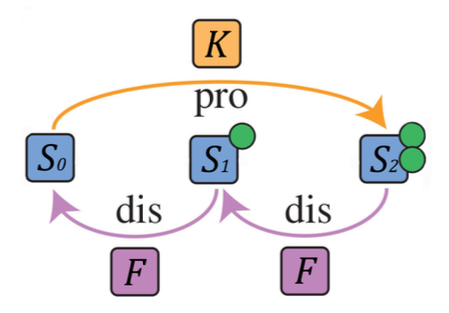
\includegraphics[width=0.4\linewidth]{pics/ex3-bifurcations.png}
	\centering
\end{figure}
\begin{align}\label{network2}
	S_{0} + K \xrightleftharpoons[ k_2 ]{k_1} KS_{0} \xrightarrow{k_3} K S_1 \xrightleftharpoons{k_4} S_2 + K \tag{$\mathcal{N}_2$} \\
	S_{2} + F \xrightleftharpoons[ k_6 ]{k_5} FS_{2} \xrightarrow{k_7} S_1 + F \xrightleftharpoons[k_9]{k_8} FS_1 \xrightarrow{k_{10}} S_0 + F \notag
\end{align}

Simplify by reversible reactions, thanks to the presesrving of bifurcations due to this opperation, studied in \cite{banaji2017}:
\begin{align}\label{network2_irr}
	S_{0} + K \xrightarrow{k_1} KS_{0} \xrightarrow{k_2} K S_1 \xrightarrow{k_3} S_2 + K \tag{$\mathcal{N}_2 / IR $} \\
	S_{2} + F \xrightarrow{k_4} FS_{2} \xrightarrow{k_5} S_1 + F \xrightarrow{k_6} FS_1 \xrightarrow{k_{7}} S_0 + F \notag
\end{align}
\end{frame}

\begin{frame}
Simplifying even further, removing reactions whose reaction vectors are linearly dependent of the original ones:

\begin{align}\label{network2_irr_s}
	S_{0} \xrightarrow{k_1} KS_{0} \xrightarrow{k_2} K S_1 \xrightarrow{k_3} S_2 \tag{$\mathcal{N}_2 / IR / S$} \\
	S_{2} + F \xrightarrow{k_4} FS_{2} \xrightarrow{k_5} F \xrightarrow{k_6} FS_1 \xrightarrow{k_{7}} S_0 + F \notag
\end{align}

And even further by removing $FS_1$,$KS_0$ and their corresponding $2$ reactions, dipping from rank $\Gamma_{\text{\ref{network2_irr_s}}}$ = 6 to rank $\Gamma_{\text{\ref{network2_irr_ss}}}$ = 4.
\begin{align}\label{network2_irr_ss}
	S_{0} \xrightarrow{k_1} KS_{1} \xrightarrow{k_2} S_2 \tag{$\mathcal{N}_2 / IR / SS$} \\
	S_{2} + F \xrightarrow{k_3} FS_{2} \xrightarrow{k_4} F \xrightarrow{k_{5}} S_0 + F \notag
\end{align}

So if $\exists$ bifurcations in \ref{network2_irr_ss} $\implies$ \ref{network2_irr_s} $\implies$ \ref{network2_irr} $\implies$ \ref{network2}.
\end{frame}

\begin{frame}
\[
	J_{\text{\ref{network2_irr_ss}}}(h,\lambda)=
	\begin{bmatrix}-\lambda h_{1}&0&0&\lambda h_{4}&0\\\lambda h_{1}&-\lambda h_{2}&0&0&0\\0&\lambda h_{2}&-\lambda h_{3}&-\lambda h_{4}&0\\0&0&-\lambda h_{3}&-\lambda h_{4}&\lambda h_{5}\\0&0&\lambda h_{3}&\lambda h_{4}&-\lambda h_{5}
	\end{bmatrix}.
\]
\[
	det(zI-J_A(h,\lambda))=z[a_0(h,\lambda)z^4+a_1(h,\lambda)z^3+a_2(h,\lambda)z^2+a_3(h,\lambda)z+a_4(h,\lambda)].
\]

And we can use the simplification above since:
$E^T = \left(1,1,1,1,1\right)$
Also, we can tell that
\[
	\forall h > 0 : a_{0}(h,\lambda)>0,\ldots,a_{4}(h,\lambda)>0\quad \text{ and } \quad\det H_{1}(h,\lambda)>0,\det H_{2}(h,\lambda)>0.
\]

Through good choices of $h$'s
\begin{align*}
	\det \text{H}_3 &=
	t^2 \lambda^6
	(
		8t^4 + 24t^3h_3 + 16t^3h_4 + 24t^2h_3^2 + \\
		23t^2h_3h_4+ 10t^2h_4^2 + 8th_3 \\
		+ 10th_3^2h_4 + 4th_3h_4^2 +
		2th_4^3 - h_3h_4 - 2h_3^2h_4^2 - h_3h_4^3
	) \\
	&= 	t^2 \lambda^6 \cdot g(t)
\end{align*}

\end{frame}

\begin{frame}
\begin{theorem}
	Through the \alert{Intermediate Value Theorem} as well
	$\implies t_1$ for which $\det \text{H}_3(t_1) = 0$, $\frac{d  \det \text{H}_3(t_1) }{dt} > 0 \implies$		
	\ref{network2_irr_ss} has bifurcations $\implies$ \ref{network2} does as well.
\end{theorem}
Now using our app:
\[
	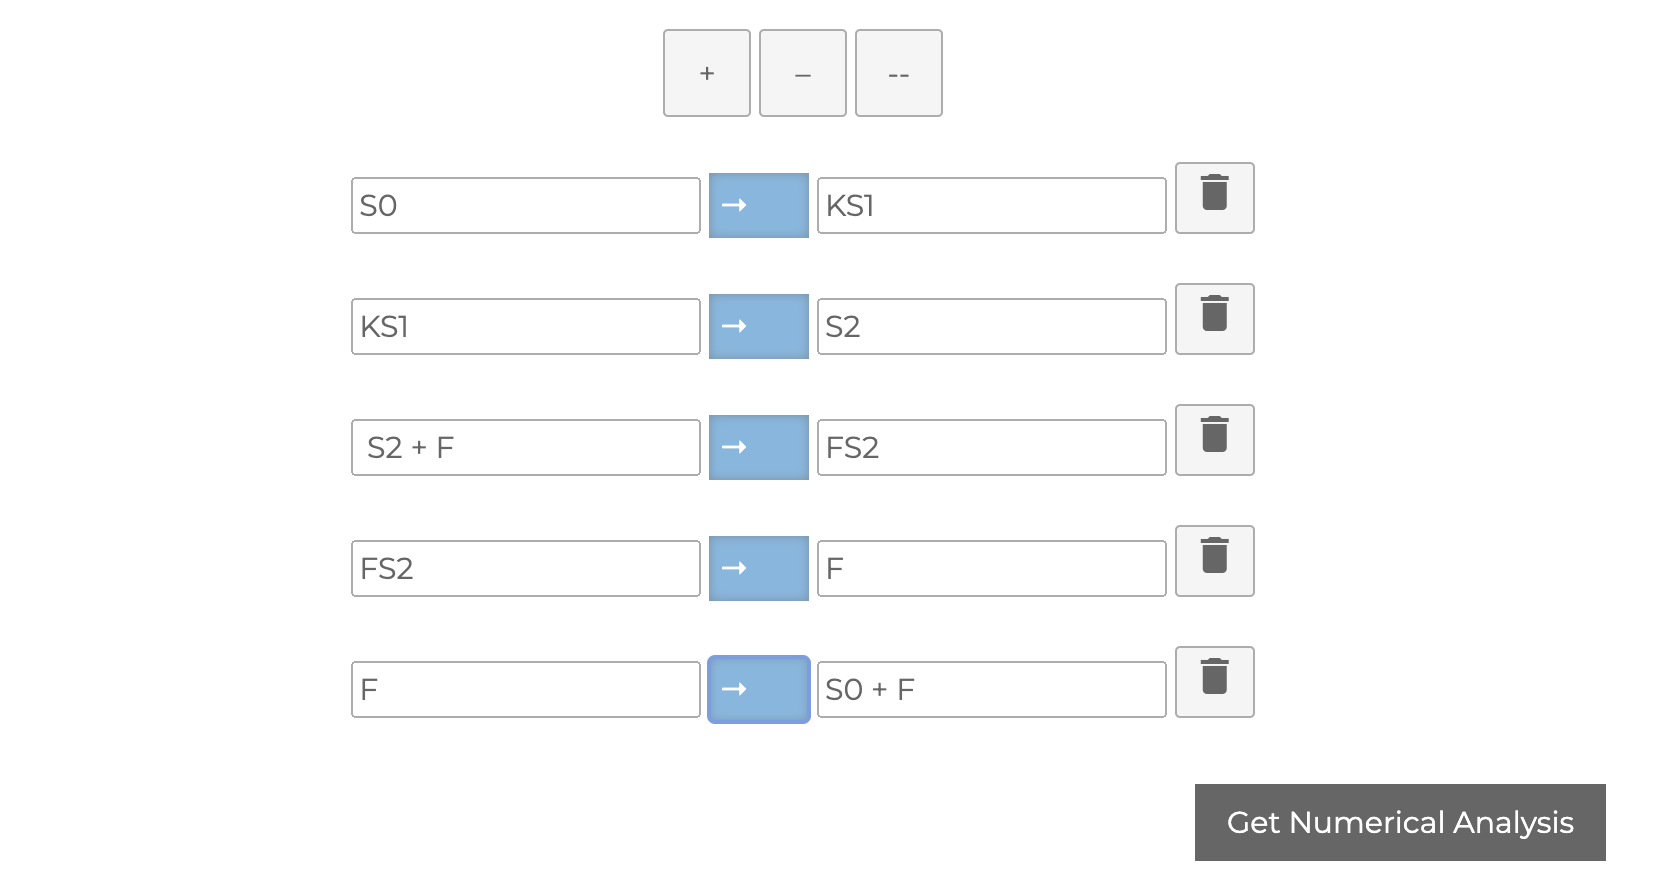
\includegraphics[width=0.4\linewidth]{pics/creca-prima-data-cand-am-scris-asta.png}
\]

\end{frame}

\begin{frame}[fragile]

\begin{figure}[H]
	\centering
	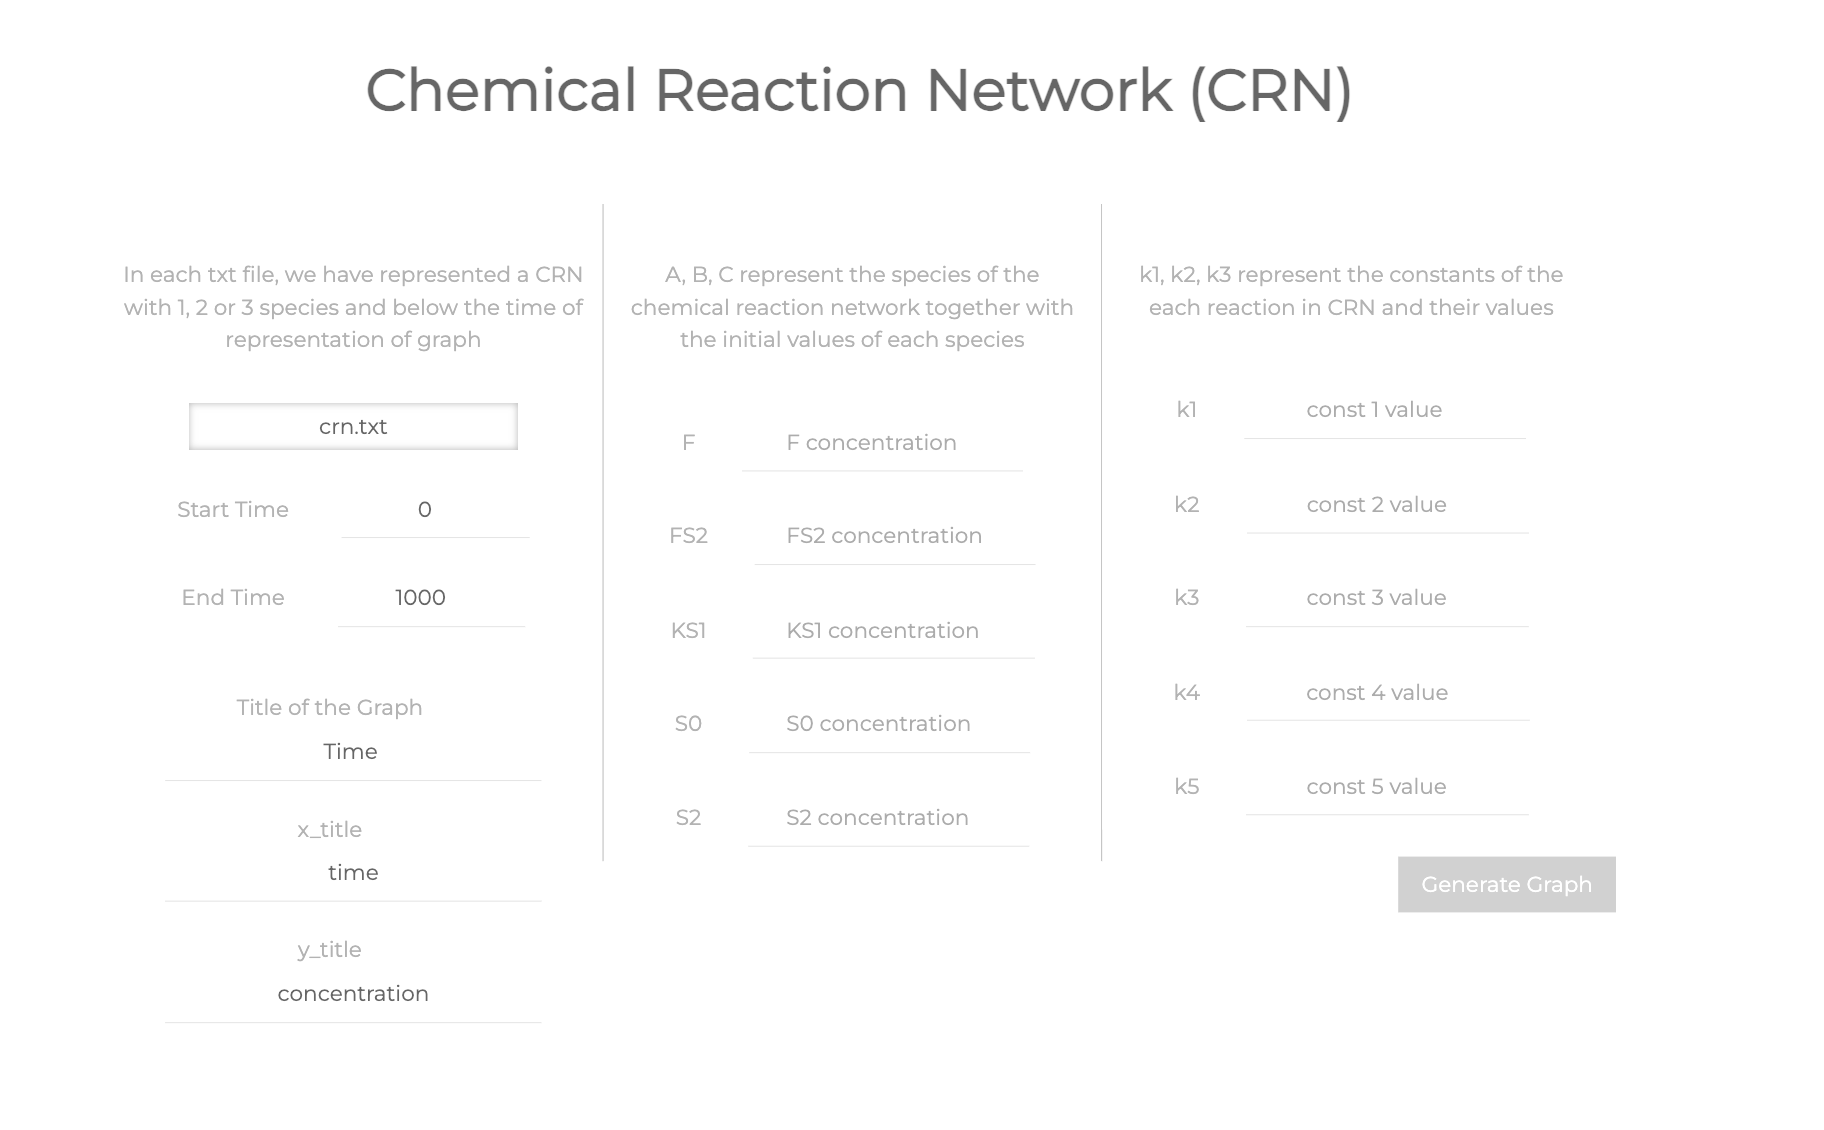
\includegraphics[width=0.4\linewidth]{pics/tsr-input.png}\\
\end{figure}

And with the initial conditions and reaction constants

{
	\small
\begin{lstlisting}
    F = 0.874108
    FS2 = 7.620157734
    KS1 = 7.620157734
    S0 = 7.270157734
    S2 = 0.6

    k1 = 0.1329759342
    k2 = 0.1329759342
    k3 = 2
    k4 = 0.1329759342
    k5 = 1
\end{lstlisting}
}

\end{frame}

\begin{frame}
outcomes the graph:

\[
	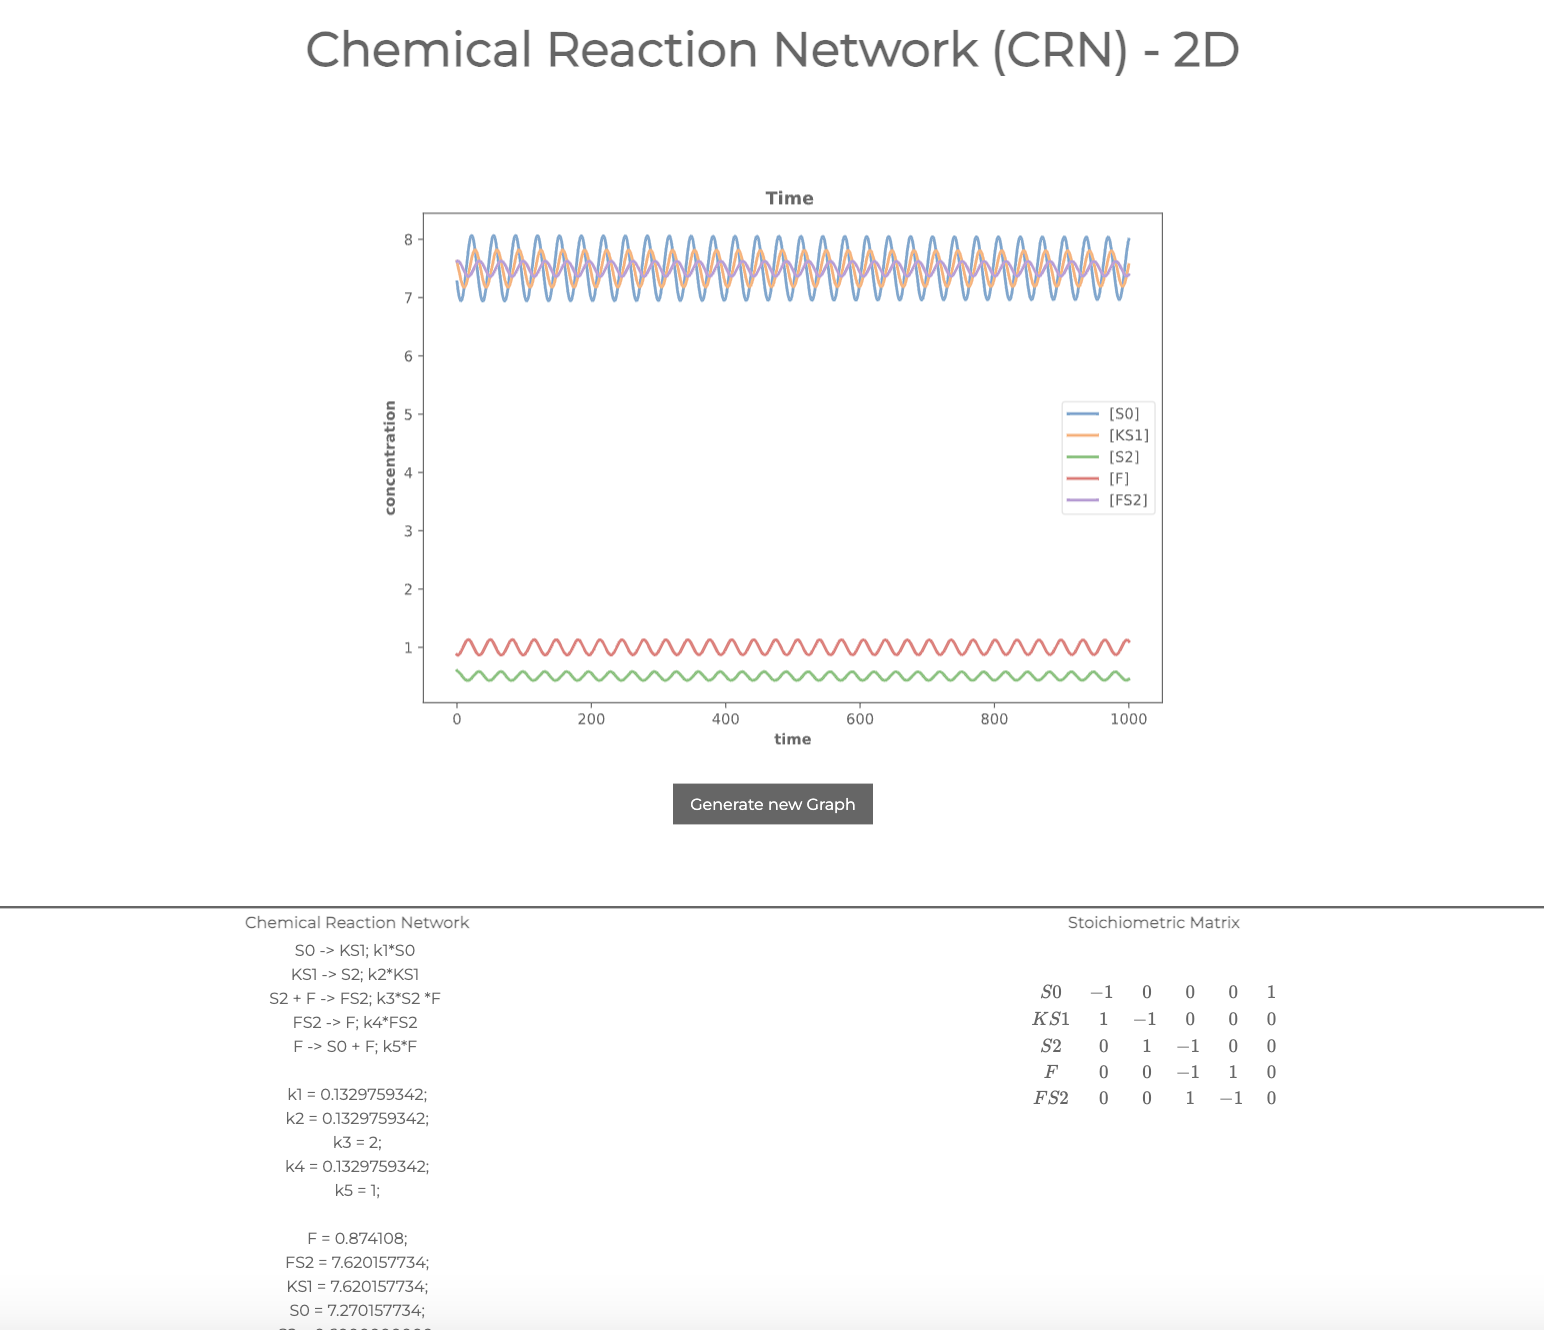
\includegraphics[width=0.5\linewidth]{pics/a-graph-indeed.png}\\
\].

\end{frame}

% --- Section 7: Case Study: Network N2 - Finding Oscillations ---
\section{$\mathcal{N}_3$}

\begin{frame}{\insertsectionhead}

\frametitle{$\mathcal{N}_3$: A Cyclic Double Phosphorylation System}
Consider the cyclic, distributive double (de)phosphorylation system
\begin{figure}[H]
	\centering
	
\includegraphics[width=0.6\linewidth]{pics/cyclic-distributive-n1.png} \\
	\caption{A Cyclic and Distributive Phosphorylation System}
\end{figure}
\begin{align*}
	S_{00} + K &\rightleftharpoons KS_{00} \rightarrow S_{10} + K & S_{10} + K &\rightleftharpoons KS_{10} \rightarrow S_{11} + K \tag{$\mathcal{N}_3$} \\
	S_{11} + F &\rightleftharpoons FS_{11} \rightarrow S_{01} + F & S_{01} + F &\rightleftharpoons FS_{01} \rightarrow S_{00} + F
\end{align*}
\end{frame}

\begin{frame}{\insertsectionhead}
\frametitle{$\mathcal{N}_3$ (Irreversible): Setup for Analysis}
Irreversible reactions which we're going to analyze:
\begin{align*}
	S_{00} + K \xrightarrow{\kappa_1} KS_{00} \xrightarrow{\kappa_3} S_{10} + K \xrightarrow{\kappa_4} KS_{10} \xrightarrow{\kappa_6} S_{11} + K \tag{$\mathcal{N}_3$}
	\\
	S_{11} + F \xrightarrow{\kappa_7} FS_{11} \xrightarrow{\kappa_9} S_{01} + F \xrightarrow{\kappa_{10}} FS_{01} \xrightarrow{\kappa_{12}} S_{00} + F \ \notag
\end{align*}
\begin{itemize}
	\item 10 species, 8 reactions.
	\item 3 conservation laws (total kinase, total phosphatase, total substrate) $\implies$ rank of Jacobian is $10-3=7$. So, effective degree $s=7$.
	\item The steady-state flux cone is a \alert{single extreme ray} $E^T = (1,1,1,1,1,1,1,1)$.
	\item We can use the $J_\lambda(h) = \lambda J_1(h)$ simplification.
\end{itemize}
\end{frame}

\begin{frame}
\[
	\begin{aligned}
		\dot{x}_{1} &= -\kappa_{1} x_{1} x_{3} - \kappa_{4} x_{1} x_{4} + \kappa_{3} x_{7} + \kappa_{6} x_{8},\\
		\dot{x}_{2} &= \kappa_{9} x_{10} - \kappa_{10} x_{2} x_{5} - \kappa_{7} x_{2} x_{6} + \kappa_{12} x_{9},\\
		\dot{x}_{3} &= -\kappa_{1} x_{1} x_{3} + \kappa_{12} x_{9},\\
		\dot{x}_{4} &= -\kappa_{4} x_{1} x_{4} + \kappa_{3} x_{7},\\
		\dot{x}_{5} &= \kappa_{9} x_{10} - \kappa_{10} x_{2} x_{5},\\
		\dot{x}_{6} &= -\kappa_{7} x_{2} x_{6} + \kappa_{6} x_{8},\\
		\dot{x}_{7} &= \kappa_{1} x_{1} x_{3} - \kappa_{3} x_{7},\\
		\dot{x}_{8} &= \kappa_{4} x_{1} x_{4} - \kappa_{6} x_{8},\\
		\dot{x}_{9} &= \kappa_{10} x_{2} x_{5} - \kappa_{12} x_{9},\\
		\dot{x}_{10} &= -\kappa_{9} x_{10} + \kappa_{7} x_{2} x_{6}.
	\end{aligned}
\]
Now there are 3 conservation laws for both networks, diminishing the rank of the Jacobian matrix to $7$. These are:
\[
	\begin{aligned}
		x_{1}+x_{7}+x_{8}&=c_{1}\\x_{2}+x_{9}+x_{10}&=c_{2}\\x_{3}+x_{4}+x_{5}+x_{6}+x_{7}+x_{8}+x_{9}+x_{10}&=c_{3}
	\end{aligned}
\]
\end{frame}

\begin{frame}
And Now with the simplifications we can obtain the relations
\begin{gather*}
	\kappa_1x_1x_3=\kappa_3x_7=\kappa_4x_1x_4=\kappa_6x_8=\kappa_7x_2x_6=\kappa_9x_{10}=\kappa_{10}x_2x_5=\kappa_{12}x_9=\lambda. \\
	\Downarrow \\
	x_{3} = \frac{\lambda}{\kappa_{1} x_{1}}, \ x_{4} = \frac{\lambda}{\kappa_{4} x_{1}}, \ x_{5} = \frac{\lambda}{\kappa_{10} x_{2}}, \ x_{6} = \frac{\lambda}{\kappa_{7} x_{2}} \\
	x_{7} = \frac{\lambda}{\kappa_{3}}, \ x_{8} = \frac{\lambda}{\kappa_{6}}, \ x_{9} = \frac{\lambda}{\kappa_{12}}, \ x_{10} = \frac{\lambda}{\kappa_{9}} \\
	\forall x_1, x_2 > 0 \\
	\Downarrow \\
	\kappa_{1} = h_{1} h_{3} \lambda, \kappa_{3} = h_{7} \lambda, \kappa_{4} = h_{1} h_{4} \lambda, \kappa_{6} = h_{8} \lambda \\
	\kappa_{7} = h_{2} h_{6} \lambda, \kappa_{9} = h_{10} \lambda, \kappa_{10} = h_{2} h_{5} \lambda, \kappa_{12} = h_{9} \lambda \\
	\text{with } h_i = \frac{1}{x_i} , i = \overline{1,10}
\end{gather*}
\end{frame}

\begin{frame}
And, $J_\lambda(h)$:
\begin{align}
	J_\lambda(h) = \lambda
	\left.\left[
		\begin{array}{rrrrrrrrrr}-2h_{1}&0&-h_{3}&-h_{4}&0&0&h_{7}&h_{3}&0&0\\0&-2h_{2}&0&0&-h_{5}&-h_{6}&0&0&h_{9}&h_{10}\\-h_{1}&0&-h_{3}&0&0&0&0&0&h_{3}&0\\-h_{1}&0&0&-h_{4}&0&0&h_{7}&0&0&0\\0&-h_{2}&0&0&-h_{5}&0&0&0&0&h_{10}\\0&-h_{2}&0&0&0&-h_{6}&0&h_{3}&0&0\\h_{1}&0&h_{3}&0&0&0&-h_{7}&0&0&0\\h_{1}&0&0&h_{4}&0&0&0&-h_{3}&0&0\\0&h_{2}&0&0&h_{5}&0&0&0&-h_{9}&0\\0&h_{2}&0&0&0&0&h_{6}&0&0&-h_{10}
	\end{array}\right.\right]
\end{align}
with $rank(J_\lambda(h)) = 7$ and characteristic polynomial is of the form:
\[
	\det\left(\mu I-J_\lambda(h)\right)=\mu^3\left(\mu^7+\lambda b_1(h)\mu^6+\ldots+\lambda^6b_6(h)\mu+\lambda^7b_7(h)\right),
\]
With $b_i(h)$ from char. poly of $J_1(h)$.
\end{frame}

\begin{frame}
Now, constructing the (simplified) Hurwitz matrices $G_i(h), i = \overline{1,6}$. Assume that at a fixed $h = h^*$ the following occur.
\begin{equation}\label{eq:hopf-conditions}
	\begin{aligned}b_{7}(h^{*})&>0and\\\det(G_1(h^*))&>0,\ldots,\det(G_5(h^*))>0and\\\det(G_6(h^*))&=0.
	\end{aligned}
\end{equation}
then, if additionally:
\[
	\exists l\in\{1,\ldots,10\} : \frac{\partial\det(G_6)}{\partial h_l}|_{h=h^*}\neq0\quad.
\]

Then ($\mathcal{N}_3$) has a simple Hopf bifurcation at $h = h^*, \forall \lambda > 0$.

$\det(G_6(h))$ has terms with both signs, so it may have roots.

In the following section we'll talk about $\det(G_6(h))$'s potential to have roots.
\end{frame}

\begin{frame}
The \textbf{Newton polytope} of that polynomial is.
\[
	\mathrm{Newt}(f)=\left\{\sum_k\alpha_k\mathbf{a}_k:\sum_k\alpha_k=1 \And \forall j\alpha_j\geq0\right\}. \forall c_k \neq 0_n
\] With Polymake \cite{Gawrilow2000}, we're able factor out $h_{10}h_7 - h_8 h_9$ in the hyper-plane intersection form of the polytope.
Doing the restriction / transformation $h_1\to t,h_2\to t,h_3\to t,h_6\to t. \implies$ can represent $\det G_6(h)$ as:
\begin{equation}\label{eq:det-g6}
	\begin{aligned}
		\det G_6(t)
		&=324t^{18}(h_{10}+h_7)(h_{10}h_7-h_8h_9)+\ldots\\&+h_{10}h_4h_5h_7h_8h_9\\&\cdot(h_{10}+h_4)(h_{10}+h_5)(h_{10}+h_7)(h_{10}+h_8)(h_{10}+h_9)\\&\cdot(h_4+h_5)(h_4+h_7)(h_4+h_8)(h_4+h_9)\\&\cdot(h_5+h_7)(h_5+h_8)(h_5+h_9)\\&\cdot(h_7+h_8)(h_7+h_9)\\&\cdot(h_8+h_9).
	\end{aligned}
\end{equation}
\end{frame}

\begin{frame}{\insertsectionhead}
\frametitle{$\mathcal{N}_3$: Transversality}
$\det G_6(0) > 0$, so if
\begin{equation}\label{cond:negative}
	h_{10}h_{7} - h_{8}h_{9} < 0, \implies \exists t_1 > 0 : \det G_6(t_1) = 0, \det G_6(t) < 0, \forall t > t_1 \text{ by the }
\end{equation}
\alert{Intermediate Value Theorem}.
So it means we've shown a root exists for $\det G_6(h)$, so a bifurcation may occur in our system.

Once a root $h^*$ for $\det G_6(h)=0$ is found (with other positive Hurwitz determinants), the transversality condition must also be checked:
$$ \frac{\partial \det(G_6(h))}{\partial h_l} \bigg|_{h=h^*} \neq 0 \quad \text{for some } l \in \{1, \dots, 10\} $$
This ensures the eigenvalues cross the imaginary axis.
\end{frame}

\begin{frame}{\insertsectionhead}
\frametitle{Where to find the bifurcations?}
Choose random for \ref{cond:negative}, \ref{eq:hopf-conditions} and using the change of variabls from $2$ slides ago, plugging into \ref{eq:det-g6}, say
\begin{gather*}
	497664+10946304t+103721056t^{2}+579850652t^{3}+2169242876t^{4} \\
	+5787611019t^{5}+113986711182t^{6}+16865933820t^{7} \\
	+18863357157t^{8}+15900121640t^{9}+9989687485t^{10} \\
	+4589099030t^{11}+1497364081t^{12}+331280824t^{13} \\
	+45135703t^{14}+2794428t^{15}-85122t^{16}-20304t^{17}-648t^{18}=0	
\end{gather*} $\implies t^* \approx 14.8$, which also verifies transversality! Getting these bifurcation values.
\begin{align*}
	x &= \left( \frac{1}{15},\frac{1}{15},\frac{1}{15},1,1,\frac{1}{15},1,1,\frac{1}{2},1 \right)^T \\
	k &= \left( 225 \lambda, \lambda, 15\lambda, 225\lambda, \lambda, 15\lambda, 2\lambda  \right)
\end{align*}
\end{frame}

\begin{frame}
\begin{figure}[H]
	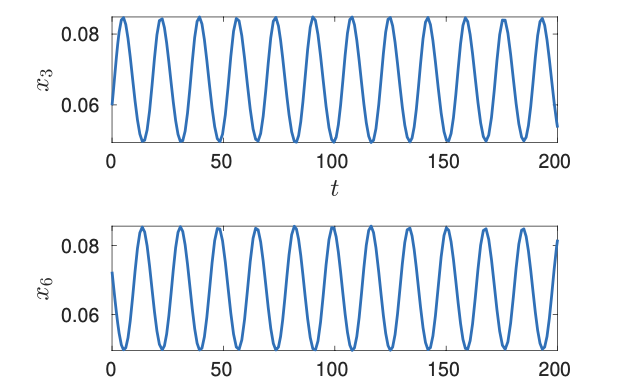
\includegraphics[width=0.9\linewidth]{pics/oscillations.png}
	\centering
	\label{fig:x3_x6_osccilations}
	\caption{Oscillations of $S00, S11$}
\end{figure}	
\end{frame}

\begin{frame}
Using inheretance results from \cite{banaji2017}, we can add back
\begin{gather*}
	KS_{00} \xrightarrow{k_2} K \\
	KS_{10} \xrightarrow{k_5} S_{10} + K \\
	FS_{11} \xrightarrow{k_8} S_{11} + F \\
	FS_{01} \xrightarrow{k_{11}} S_{01} + F
\end{gather*}
Getting, different $k$'s and initial values for bifurcations.
% make them in a line instead of collumn
\begin{figure}[H]
	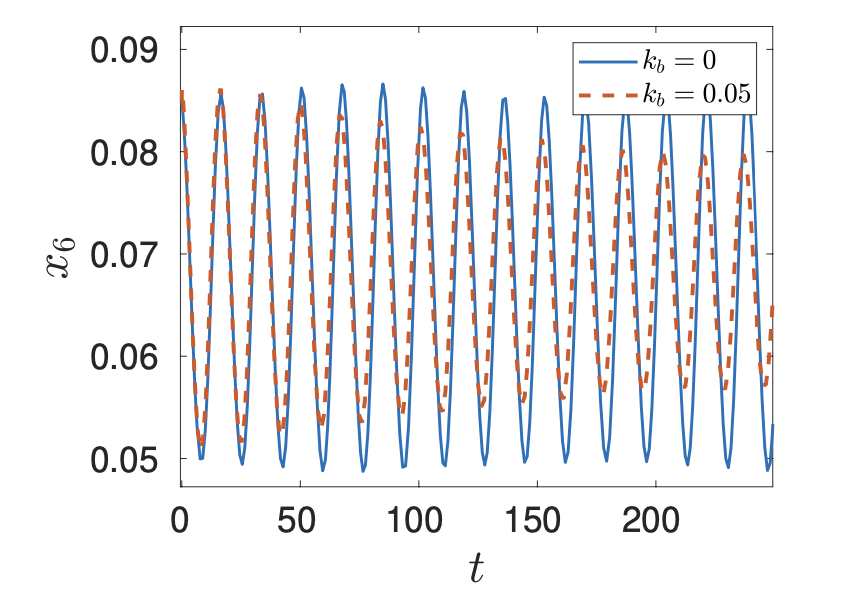
\includegraphics[width=0.3\linewidth]{pics/oscillations-full-network.png}
	\centering
	\label{fig:full_net_oscillations}
	\caption{\tiny Oscillations of the full $\mathcal{N}_3$ network}
\end{figure}
\end{frame}

\begin{frame}
\begin{theorem}
	Network $\mathcal{N}_3$ admits Hopf bifurcations for the aforementioned rate constants and initial conditions.
\end{theorem}

I've also had the
\end{frame}

\section{App presentation}

\begin{frame}
I've also had the chance of contributing a couple commits to \href{https://github.com/sys-bio/roadrunner}{libroadrunner}, the library used for plotting this:

\[
	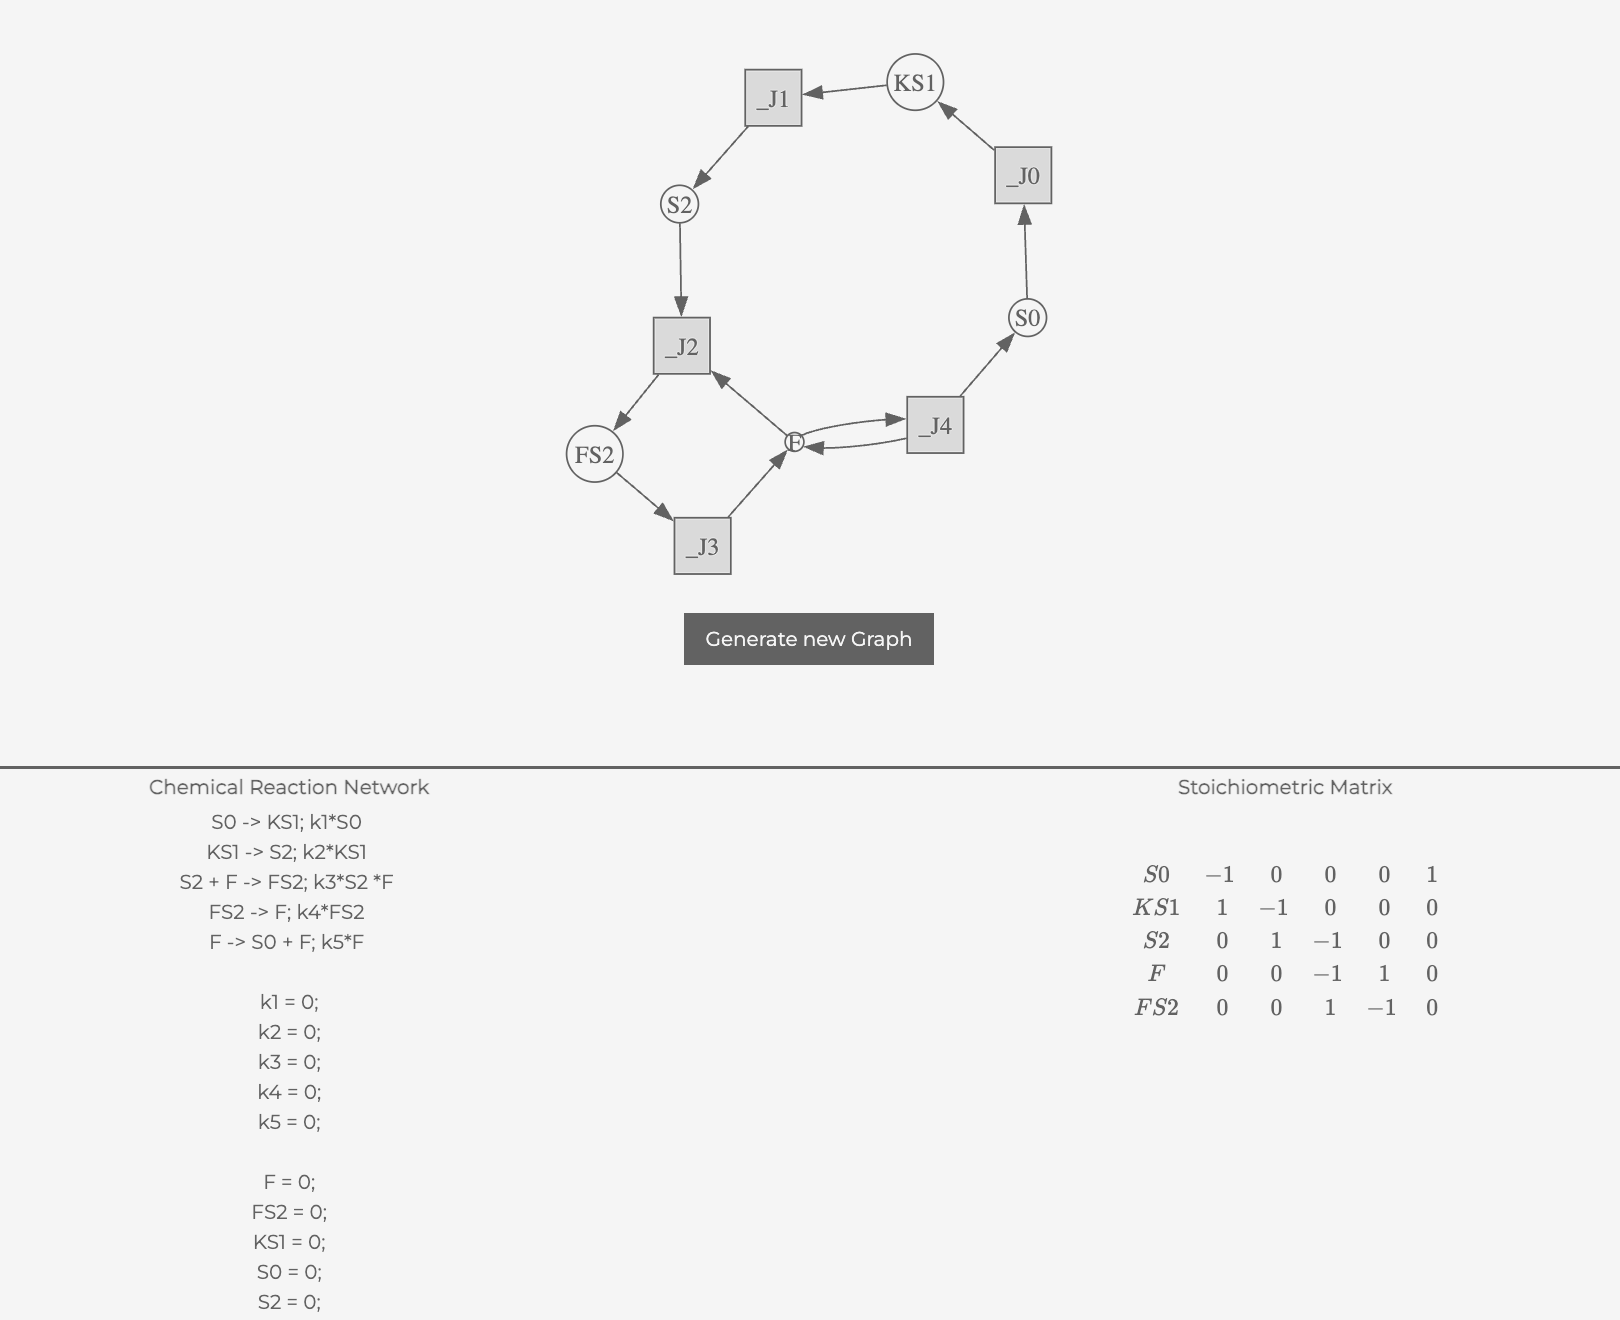
\includegraphics[width=0.5\linewidth]{pics/dsr-graph.png}
\].

So that if could be used inside this web-app, and not just a Python magic environment.

\end{frame}

\begin{frame}
We can also this $3D$ phase potrait.
\[
	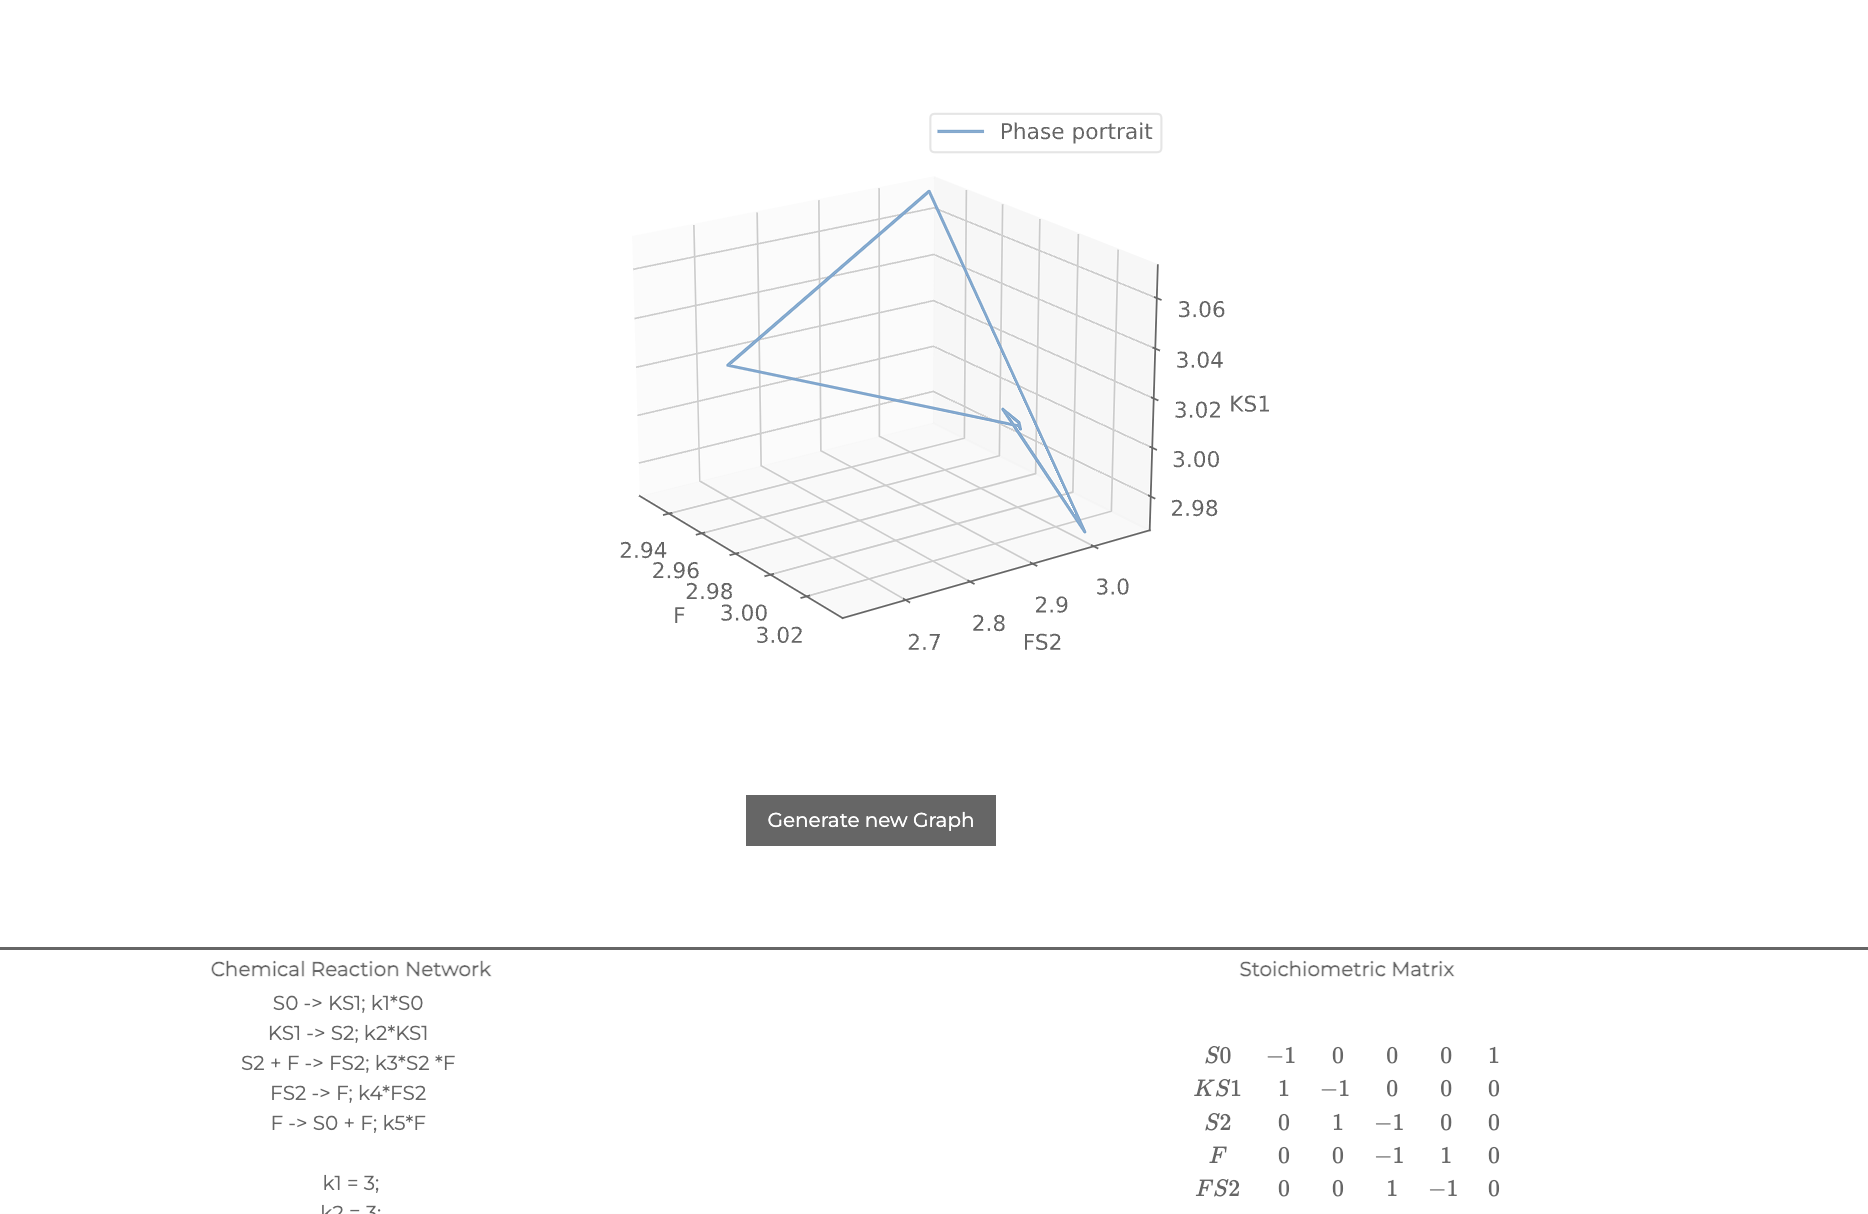
\includegraphics[width=0.5\linewidth]{pics/3D phase portrait.png}
\].

\end{frame}

% --- Section 8: Conclusion ---
\section{Conclusion}

\begin{frame}{\insertsectionhead}
\frametitle{Summary: Unveiling Chemical Networks}
\begin{itemize}
	\item Hopf bifurcations are critical for understanding how \alert{oscillations} arise in CRNs.
	\item This is vital for (de)phosphorylation networks, which underpin cellular signaling and control.
	\item Proving existence/absence of Hopf involves:
		\begin{enumerate}
			\item ODE model $\to$ Equilibria $\to$ Jacobian $J$.
			\item Characteristic polynomial of $J$.
			\item Routh-Hurwitz determinants ($\Delta_k$) to check stability and Hopf conditions (esp. $\Delta_{s-1}=0$, $\Delta_{s-2}>0, \dots, \Delta_1>0, a_s>0$, transversality).
		\end{enumerate}
	\item \alert{Convex parameterization} and \alert{single extreme ray} analysis can greatly simplify complex CRNs.
	\item We saw Network $\mathcal{N}_1$ (basic cycle) \alert{cannot} have Hopf bifurcations.
	\item We saw Networks $\mathcal{N}_2, \mathcal{N}_3$ which \alert{can} have them.
\end{itemize}
\end{frame}

\begin{frame}[plain]
\centering
\vfill
\Huge Thank You!
\vfill
Questions? \\
\vfill
\end{frame}

\begin{frame}
\frametitle{Bibliography}
\printbibliography
\end{frame}

\end{document}
